\documentclass[11pt,a4paper]{article}

% --- Packages ---
\usepackage[margin=2.5cm]{geometry}
\usepackage{amsmath}
\usepackage{amssymb}
\usepackage{siunitx}
\usepackage{booktabs}
\usepackage{graphicx}
\usepackage{subcaption}
\usepackage{xcolor}
\usepackage[colorlinks=true,linkcolor=blue!60!black,citecolor=blue!60!black,urlcolor=blue!60!black]{hyperref}

\sisetup{separate-uncertainty=true}
\graphicspath{{figures/}}

% --- Title ---
\title{Simulation Results: GaAs L3 Photonic Crystal Cavity\\Design and Characterization}
\author{Jonah Lux}
\date{April 2026}

\begin{document}
\maketitle

%% ============================================================
%%  ABSTRACT
%% ============================================================
\begin{abstract}
We present guided-mode expansion (GME) simulations of GaAs air-bridge L3 photonic crystal cavities at three optimization levels: a 1-hole optimized design ($Q \approx 2 \times 10^5$), a 3-hole globally optimized design ($Q \approx 1.44 \times 10^6$), and an extended areal optimization ($Q \approx 4.4 \times 10^7$). For each design we perform systematic parameter sweeps of hole radius, sidewall taper angle, native oxide thickness, oxide consumption ratio, hole ellipticity, and random oxide disorder. The results map the sensitivity of the quality factor and resonance wavelength to each fabrication imperfection, establishing quantitative benchmarks for interpreting experimental measurements. These simulations directly inform the layout of a GaAs characterization chip in which radius sweeps, row-number sweeps, and paired designs of different optimization levels serve as differential probes of distinct loss channels.
\end{abstract}

%% ============================================================
%%  1. INTRODUCTION
%% ============================================================
\section{Introduction}
\label{sec:introduction}

Photonic crystal (PhC) cavities confine light to mode volumes on the order of a cubic wavelength by exploiting a photonic bandgap---a frequency range in which propagation is forbidden by the periodic dielectric structure~\cite{joannopoulos2008}. Among the many cavity geometries, the L3 cavity---formed by removing three holes in a row from a triangular lattice of air holes in a thin dielectric slab---has become a workhorse design because of its relatively high quality factor ($Q$), small mode volume, and compatibility with planar fabrication~\cite{akahane2003}.

The quality factor of an L3 cavity can be increased by orders of magnitude through gentle optimization of the positions of the holes nearest to the cavity. Akahane~et~al.\ demonstrated that shifting the two end-hole pairs outward by $\sim 0.2a$ reduces far-field radiation loss by softening the mode envelope at the cavity boundary~\cite{akahane2003}. Subsequent work by Minkov and Savona showed that global optimization over three or more hole pairs yields $Q > 10^6$ by cancelling leaky Fourier components that sequential single-parameter sweeps miss~\cite{minkov2014}. Ultra-high-$Q$ designs involving dozens of shifted holes have reached $Q > 10^7$ in simulation, although fabrication disorder limits experimental values to $Q_\mathrm{exp} \lesssim 5 \times 10^6$ even in the best silicon devices~\cite{asano2021,vasco2020}.

Our platform is GaAs rather than silicon, motivated by the integration of self-assembled InAs quantum dots (QDs) that emit near \SI{970}{nm}. GaAs presents distinct challenges: a smaller bandgap energy, higher surface recombination velocity, and susceptibility to native oxide formation upon air exposure. Understanding how native oxide growth, sidewall taper from dry etching, and hole-radius variations affect the cavity $Q$ is therefore essential before fabrication.

In this report we use the \texttt{legume} package~\cite{legume}, which implements the guided-mode expansion (GME) method, to simulate three L3 cavity designs of increasing optimization level. We sweep the key fabrication-sensitive parameters and present the results as a reference for designing and interpreting a GaAs characterization chip.


%% ============================================================
%%  2. CAVITY DESIGN
%% ============================================================
\section{Cavity Design}
\label{sec:design}

\subsection{Baseline Parameters}
\label{sec:baseline}

All simulations share the baseline parameters listed in Table~\ref{tab:baseline}. The guided-mode expansion uses a reciprocal-space truncation of $g_\mathrm{max} = 2$ (in units of $2\pi/a$) with the ``truncate by type'' (tbt) scheme, 52 guided modes, and a $16 \times 10$ supercell.\footnote{The refractive index used in the simulations is $n_\mathrm{GaAs} = 3.46$, corresponding to GaAs at \SI{970}{nm} at room temperature.}

\begin{table}[htbp]
  \centering
  \caption{Baseline simulation parameters.}
  \label{tab:baseline}
  \begin{tabular}{@{}llS[table-format=3.2]l@{}}
    \toprule
    Parameter & Symbol & {Value} & Unit \\
    \midrule
    Lattice constant   & $a$          & 250    & \si{nm} \\
    Hole radius        & $r$          & 75     & \si{nm} \\
    Radius ratio       & $r/a$        & 0.30   & --- \\
    Slab thickness     & $d$          & 170    & \si{nm} \\
    Thickness ratio    & $d/a$        & 0.68   & --- \\
    GaAs refractive index & $n_\mathrm{GaAs}$ & 3.46 & --- \\
    Oxide refractive index & $n_\mathrm{ox}$ & 1.72 & --- \\
    Supercell size     & $N_x \times N_y$ & \multicolumn{2}{l}{$16 \times 10$} \\
    \bottomrule
  \end{tabular}
\end{table}

\subsection{One-Hole Optimized Design}
\label{sec:1hole}

The simplest optimization shifts only the nearest end-hole pair (S1) outward along the cavity axis by $\mathrm{dx}_1 = 0.17964\,a$ (\SI{44.9}{nm}). This yields a theoretical quality factor of $Q_{1\mathrm{h}} = \num{198852}$ at a resonance wavelength of $\lambda_0 = \SI{970.7}{nm}$. The approach follows Akahane et al.~\cite{akahane2003}: a gentle Gaussian-like envelope is imposed on the cavity mode by pushing the end holes outward, reducing the amplitude of leaky wave-vector components above the light line.

\subsection{Three-Hole Optimized Design}
\label{sec:3hole}

A global optimization over the three nearest end-hole pairs (S1, S2, S3) reaches a substantially higher quality factor. Using gradient-based optimization (30 epochs, step size 0.02) following the methodology of Minkov and Savona~\cite{minkov2014}, we obtain:
\begin{align}
  \mathrm{dx}_1 &= 0.27239\,a \;(\SI{68.1}{nm}), \notag \\
  \mathrm{dx}_2 &= 0.21982\,a \;(\SI{55.0}{nm}), \label{eq:3hole_shifts} \\
  \mathrm{dx}_3 &= 0.00000\,a, \notag
\end{align}
yielding $Q_{3\mathrm{h}} = \num{1438926}$ at $\lambda_0 = \SI{973.1}{nm}$---a factor of 7.2 improvement over the 1-hole design.

\subsection{Extended Areal Optimization}
\label{sec:extended}

Extending the optimization to 15 parameters---4 row-0 shifts ($\mathrm{dx}$ only), 3 row-1 shifts ($\mathrm{dx}$ and $\mathrm{dy}$), and 3 row-2 shifts ($\mathrm{dx}$ and $\mathrm{dy}$)---reaches $Q_\mathrm{ext} = \num{43715163}$ at $\lambda_0 = \SI{978.4}{nm}$ (100 epochs, step size 0.005, parameter bounds $\pm 0.25a$). This value is \emph{unrealistic experimentally}: fabrication disorder limits real devices to $Q_\mathrm{exp} \lesssim 5 \times 10^6$~\cite{asano2021}. We retain the extended design as a \textbf{sensitivity canary}---its extreme sensitivity to any geometric perturbation makes it a powerful probe for detecting fabrication imperfections on the characterization chip.

\subsection{Design Comparison}
\label{sec:comparison}

Table~\ref{tab:designs} summarizes the three designs. The relationship between design $Q$ and experimental $Q$ is governed by:
\begin{equation}
  \frac{1}{Q_\mathrm{exp}} = \frac{1}{Q_\mathrm{design}} + \frac{1}{Q_\mathrm{disorder}} + \frac{1}{Q_\mathrm{absorption}}
  \label{eq:disorder}
\end{equation}
When $Q_\mathrm{design} \gg Q_\mathrm{disorder}$, the measured $Q$ is dominated by disorder and becomes approximately design-independent. The three optimization levels thus probe different regimes: the 1-hole design is sensitive to both design and disorder losses, the 3-hole design is primarily disorder-limited, and the extended design is overwhelmingly disorder-limited. By comparing measurements across all three, we can separate the contributions of different loss channels.

\begin{table}[htbp]
  \centering
  \caption{Comparison of the three L3 cavity optimization levels.}
  \label{tab:designs}
  \begin{tabular}{@{}lccc@{}}
    \toprule
    & 1-Hole & 3-Hole & Extended \\
    \midrule
    Degrees of freedom & 1 & 3 & 15 \\
    $Q_\mathrm{design}$        & \num{198852}   & \num{1438926}   & \num{43715163} \\
    $\lambda_0$ (\si{nm})      & 970.7          & 973.1           & 978.4 \\
    $Q$ improvement vs.\ 1-hole & $1\times$     & $7.2\times$     & $220\times$ \\
    Fabrication feasibility     & High           & High            & Research only \\
    \bottomrule
  \end{tabular}
\end{table}

\begin{figure}[htbp]
  \centering
  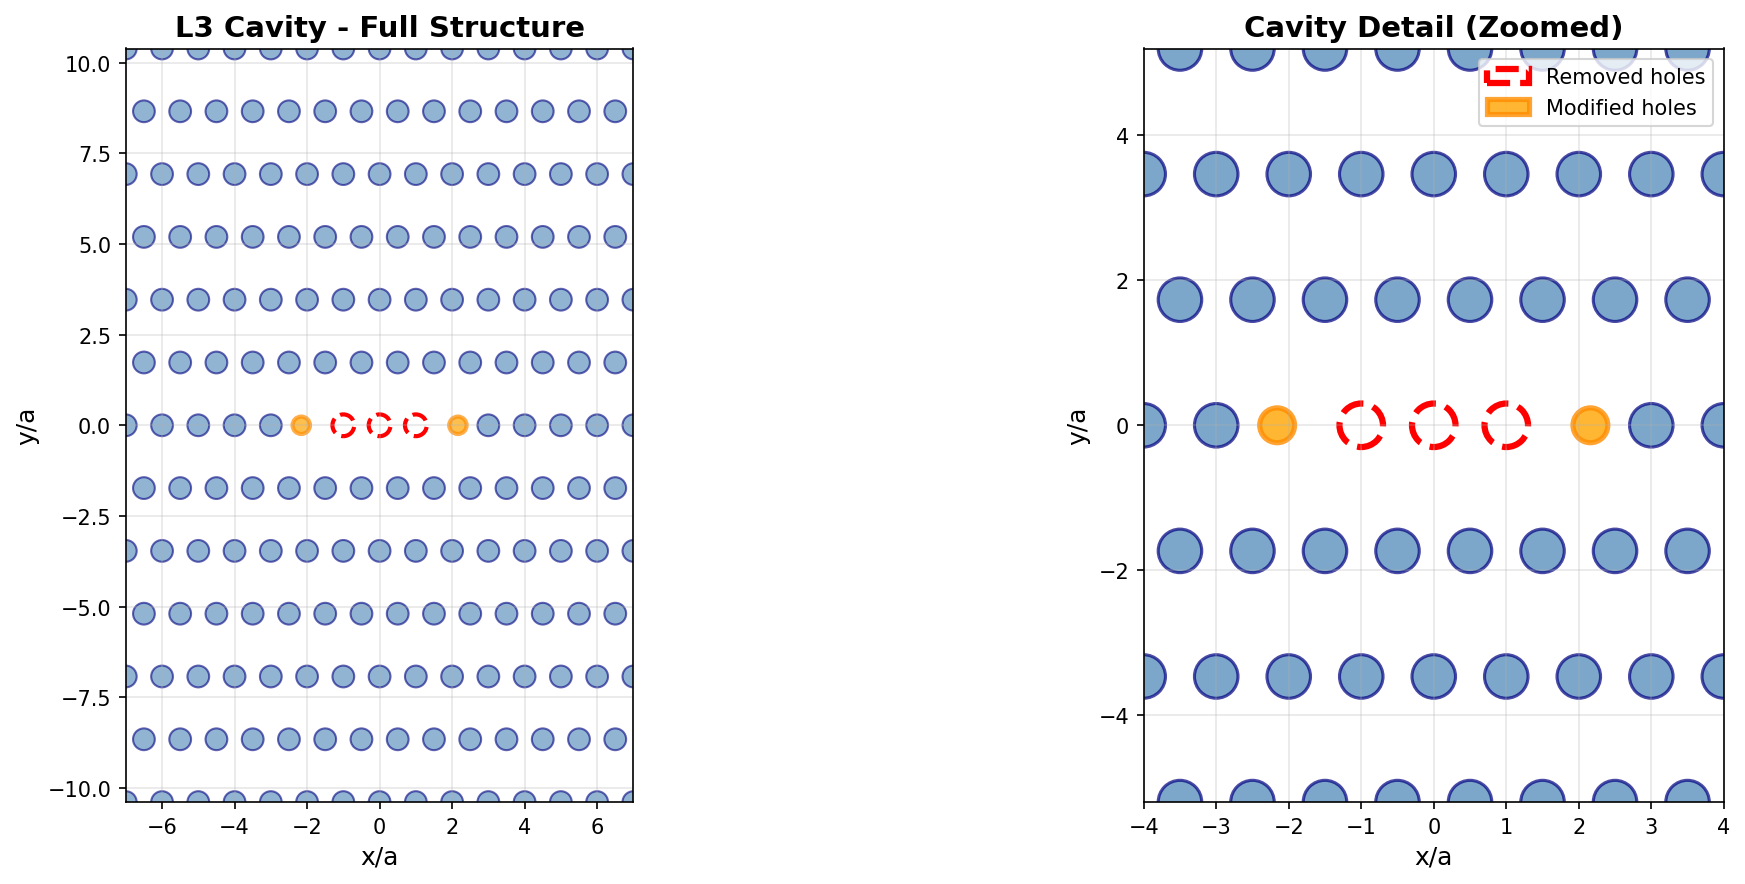
\includegraphics[width=0.55\textwidth]{../l3_structure.png}
  \caption{Schematic of the GaAs L3 photonic crystal cavity. Three holes are removed from the triangular lattice to form the cavity. The nearest end-hole pairs (S1, S2, S3) are shifted outward along the cavity axis to optimize the quality factor.}
  \label{fig:l3_schematic}
\end{figure}


%% ============================================================
%%  3. SIMULATION RESULTS
%% ============================================================
\section{Simulation Results}
\label{sec:results}

% ----------------------------------------------------------
%  3.1  Q vs. Hole Radius
% ----------------------------------------------------------
\subsection{Quality Factor vs.\ Hole Radius}
\label{sec:radius}

We sweep the hole radius from $r = \SI{73}{nm}$ to \SI{77}{nm} in \SI{1}{nm} steps at zero taper and zero oxide (Figure~\ref{fig:Q_vs_r}).

\begin{figure}[htbp]
  \centering
  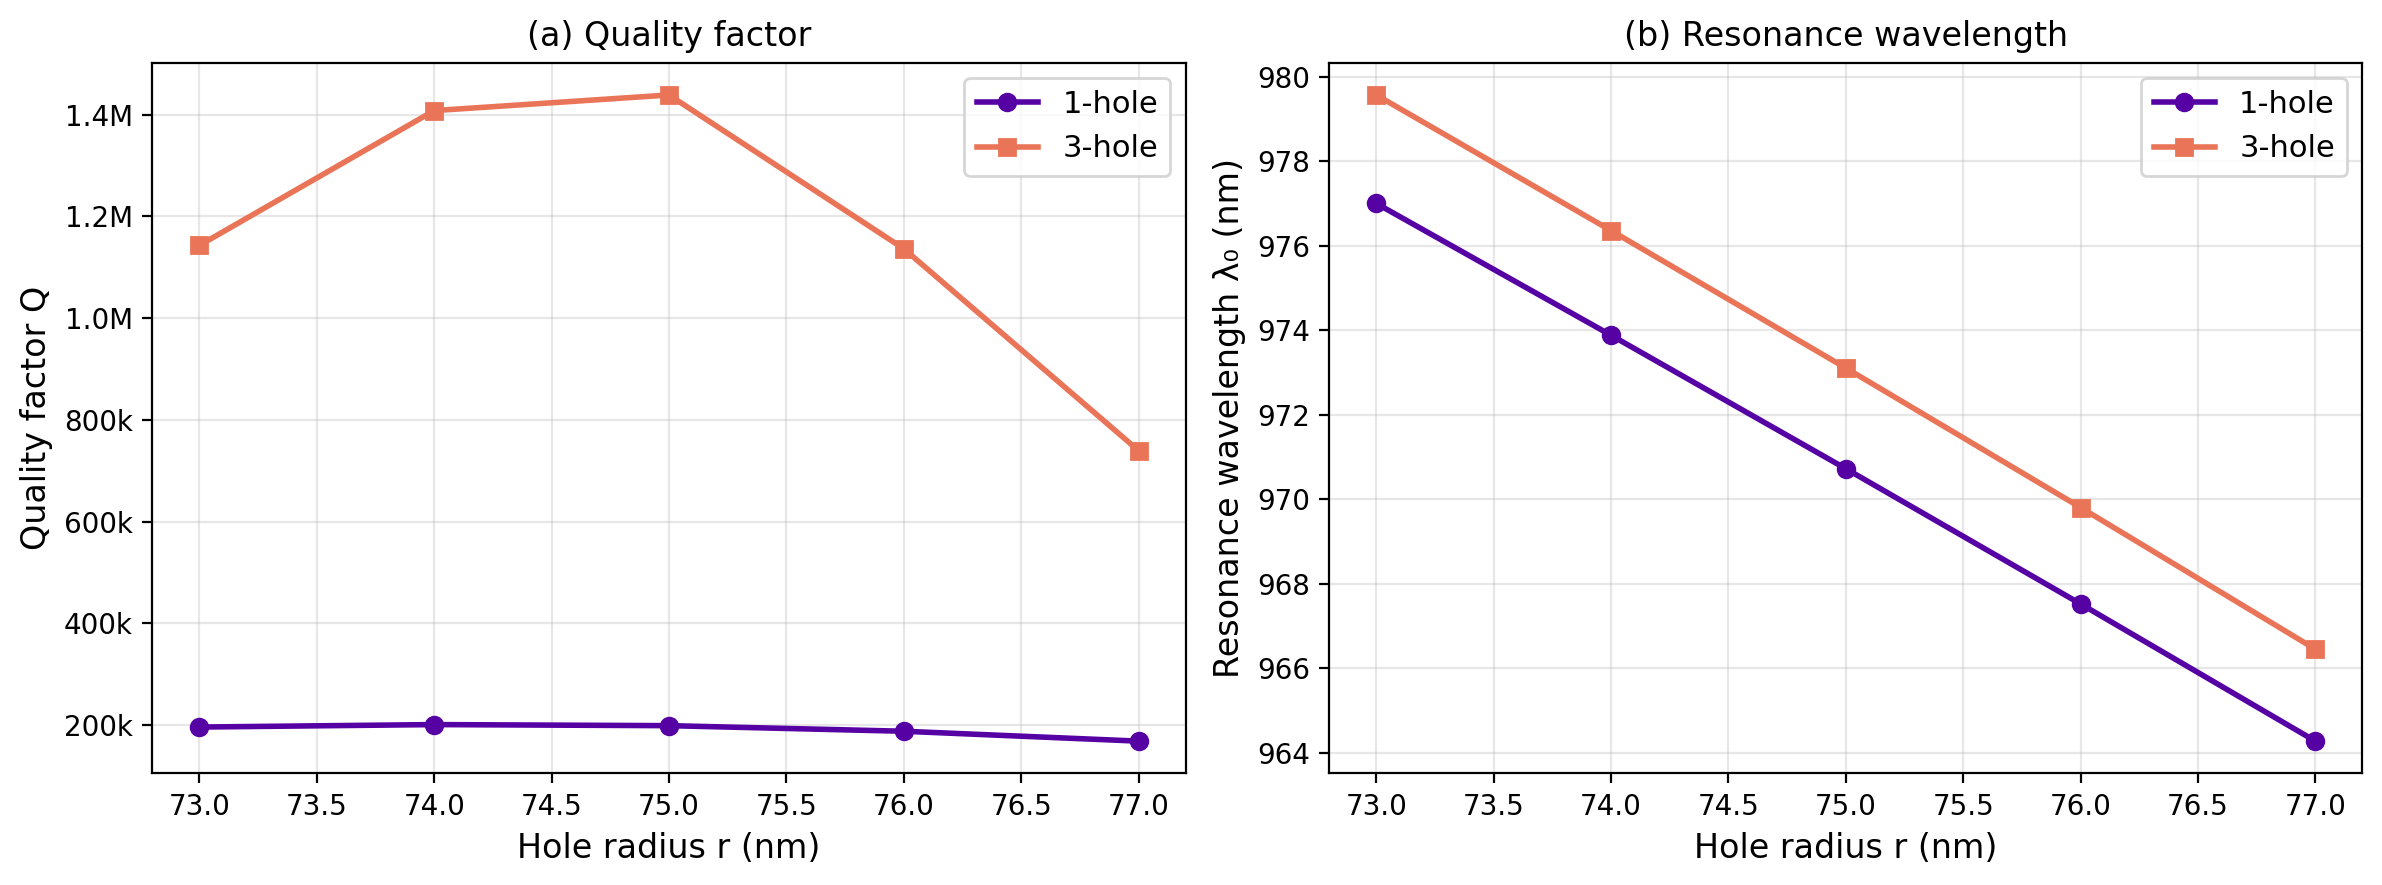
\includegraphics[width=\textwidth]{fig_Q_vs_radius.png}
  \caption{Quality factor and resonance wavelength as functions of hole radius for the 1-hole and 3-hole optimized designs.}
  \label{fig:Q_vs_r}
\end{figure}

The 1-hole design exhibits a broad $Q(r)$ plateau: $Q$ varies by only $\sim$17\% over the \SIrange{73}{77}{nm} range, peaking at $r = \SI{74}{nm}$ ($Q = \num{200982}$). In contrast, the 3-hole design has a much sharper peak at $r = \SI{75}{nm}$ ($Q = \num{1438926}$), dropping by 21\% at $r = \SI{74}{nm}$ and 49\% at $r = \SI{77}{nm}$. This sharpness is the price of high optimization: the delicate far-field cancellation achieved by the globally optimized hole shifts is finely tuned to a specific radius.

The wavelength shifts approximately linearly at $\sim$\SI{3.2}{nm} per \si{nm} of radius change for both designs. \textbf{Fabrication implication:} a measured wavelength immediately constrains the actual fabricated radius to within $\pm \SI{1}{nm}$, independent of any $Q$ degradation.


% ----------------------------------------------------------
%  3.2  Q vs. Sidewall Taper Angle
% ----------------------------------------------------------
\subsection{Quality Factor vs.\ Sidewall Taper Angle}
\label{sec:taper}

Dry etching of GaAs produces holes with non-vertical sidewalls. We model this as a conical taper: the hole radius varies linearly from $r_\mathrm{top} = r - (d/2)\tan\theta$ at the top surface to $r_\mathrm{bot} = r + (d/2)\tan\theta$ at the bottom, where $\theta$ is the taper angle. In the GME simulation the tapered hole is discretized into 24 slices.

Figure~\ref{fig:Q_vs_taper_all} shows $Q$ and wavelength vs.\ taper angle for all three designs. The extended design drops from \num{43.7e6} to \num{3.4e6} at just \SI{1}{\degree}, losing 92\% of its $Q$. The 3-hole design retains 70\% at \SI{1}{\degree} but drops to 31\% by \SI{2}{\degree}. The 1-hole design is the most robust, retaining 79\% at \SI{1}{\degree}. By \SI{5}{\degree}, all three designs converge to $Q \sim \numrange{16000}{113000}$, meaning taper becomes the dominant loss mechanism regardless of optimization level.

The physical mechanism is that taper breaks the vertical mirror symmetry of the slab, coupling the TE-like cavity mode to TM-like radiation modes. This opens an out-of-plane loss channel absent for straight holes. The wavelength redshifts at $\sim$\SI{2}{nm}/degree because tapered holes contain less air, increasing the effective index.

\begin{figure}[htbp]
  \centering
  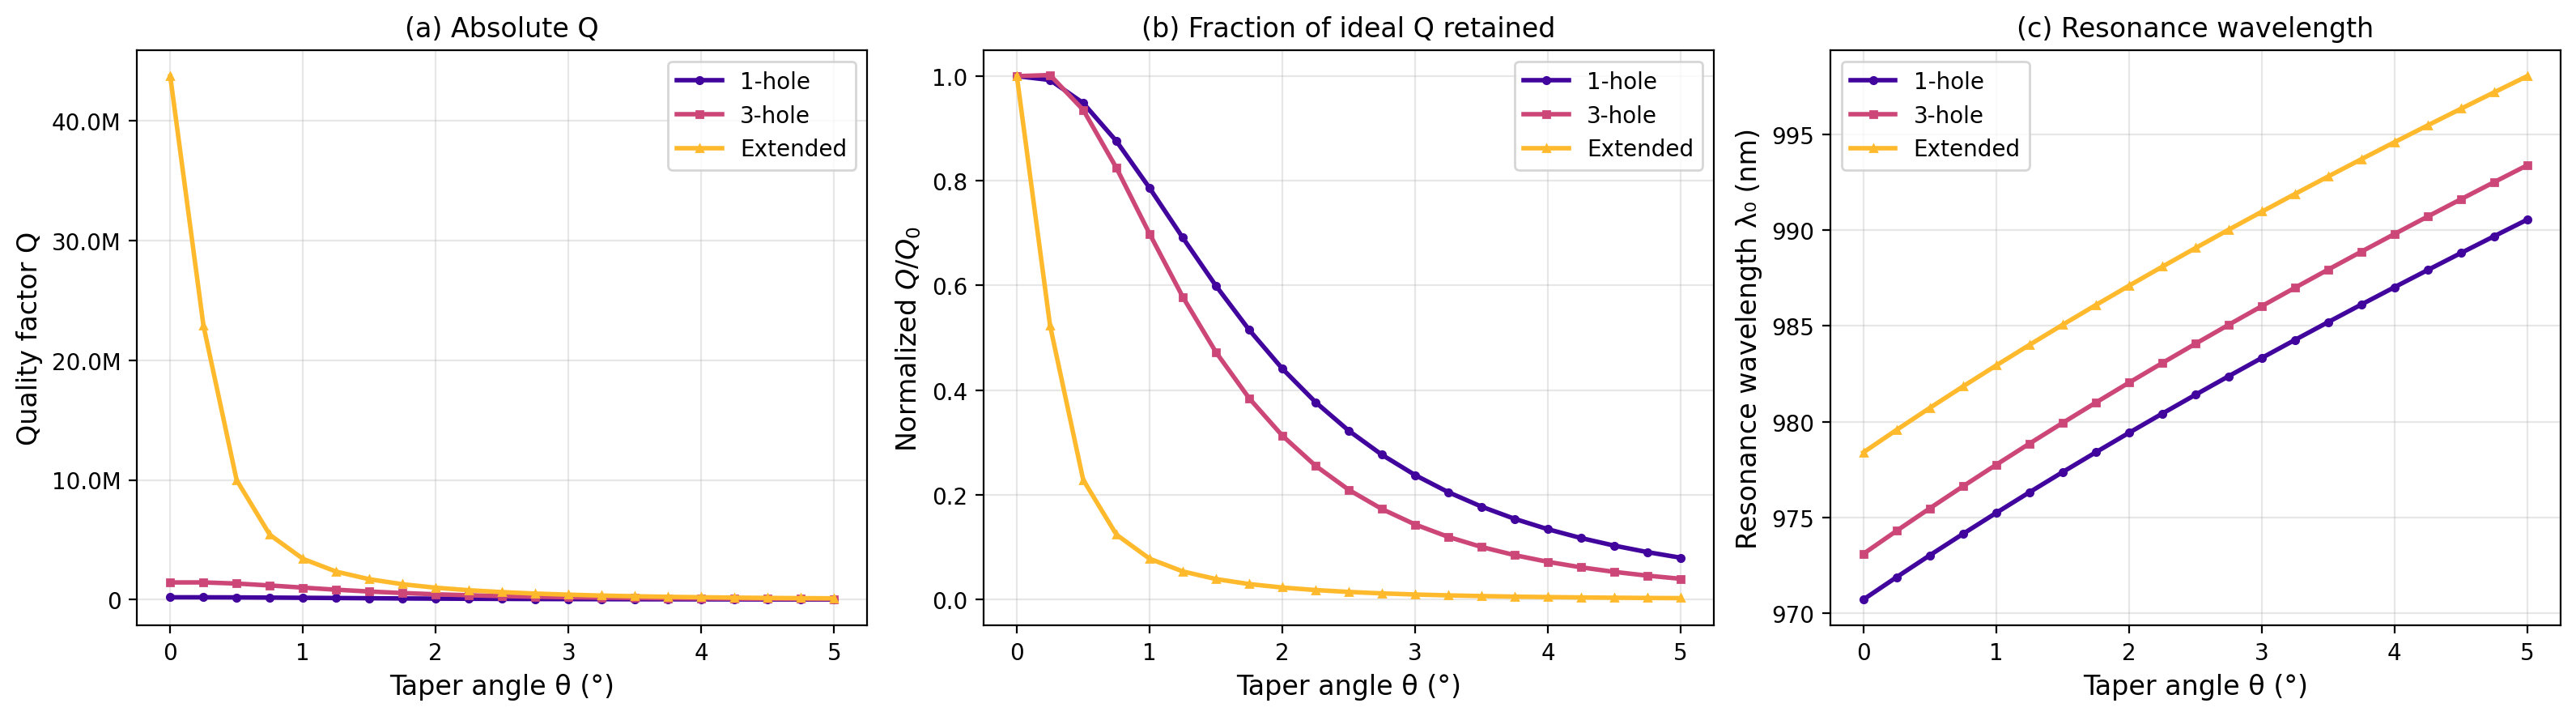
\includegraphics[width=\textwidth]{fig_Q_vs_taper_combined.png}
  \caption{Quality factor and resonance wavelength vs.\ sidewall taper angle for all three cavity designs at $r = \SI{75}{nm}$.}
  \label{fig:Q_vs_taper_all}
\end{figure}

Figure~\ref{fig:Q_vs_taper_multiradius} shows the 1-hole design at five radii. At large taper angles all radii converge, confirming that taper dominates over radius mismatch. \textbf{Fabrication implication:} if measured $Q$ values for the 1-hole and 3-hole designs are both well below simulation and their ratio approaches unity, taper is likely the dominant loss channel.

\begin{figure}[htbp]
  \centering
  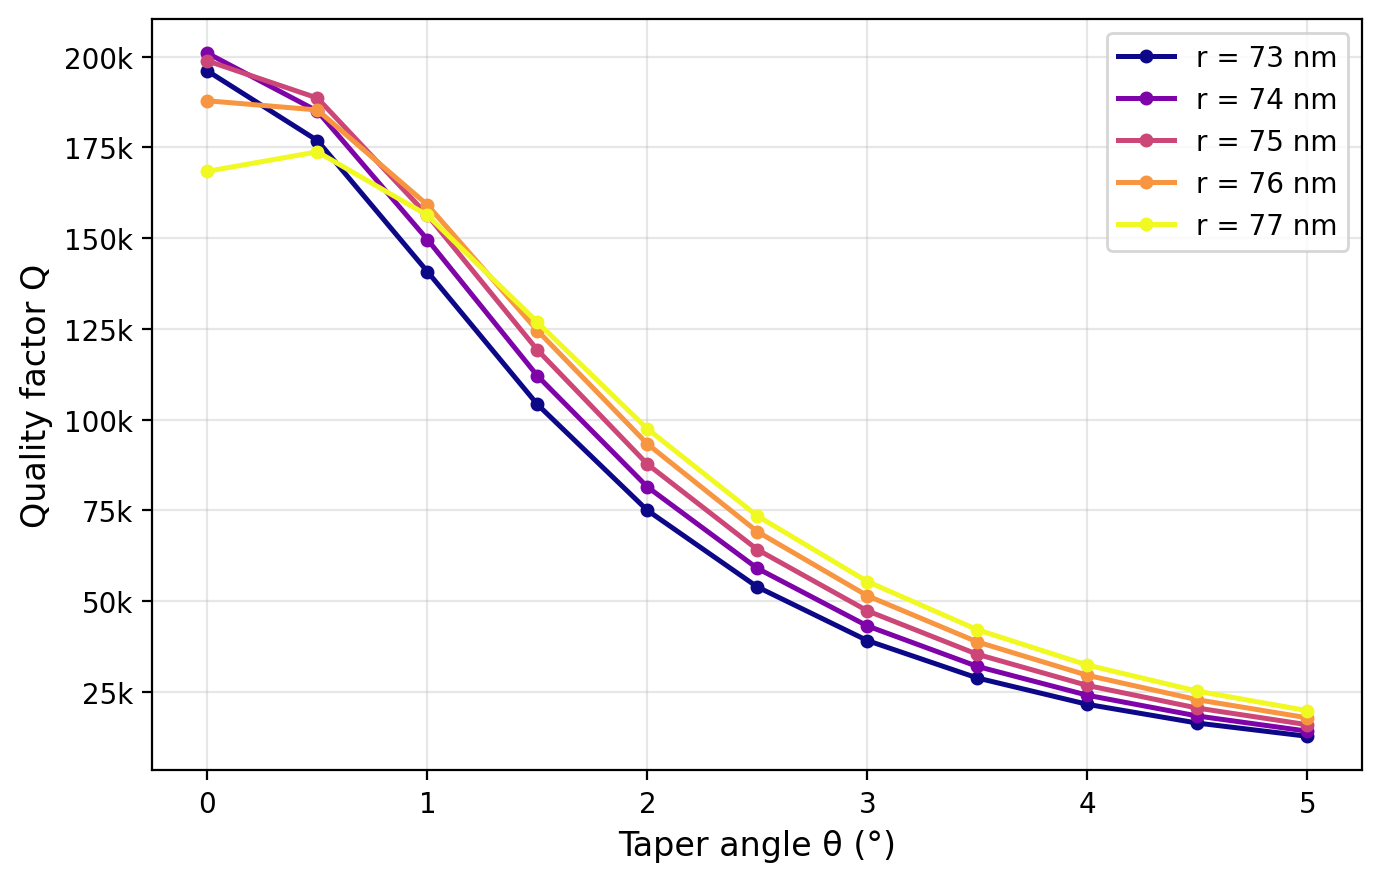
\includegraphics[width=0.7\textwidth]{fig_Q_vs_taper_multiradius.png}
  \caption{Quality factor vs.\ sidewall taper angle for the 1-hole design at five hole radii. Convergence at large angles confirms taper dominance.}
  \label{fig:Q_vs_taper_multiradius}
\end{figure}


% ----------------------------------------------------------
%  3.3  Piecewise Taper
% ----------------------------------------------------------
\subsection{Piecewise Taper Heatmaps}
\label{sec:piecewise}

Real etched holes may have asymmetric taper profiles---the top and bottom half-angles need not be equal. We explore this by independently varying the top and bottom taper angles from \SI{-3}{\degree} to \SI{5}{\degree} (Figure~\ref{fig:piecewise}). The 1-hole design shows a broad high-$Q$ region around zero taper with approximate symmetry along the diagonal (equal top and bottom angle). The 3-hole and extended designs show progressively sharper peaks centered at $(0^\circ, 0^\circ)$, confirming their higher sensitivity.

\textbf{Fabrication implication:} a negative taper angle (undercut) is as damaging as an overcut, so there is no ``safe direction'' for taper error. The heatmap also reveals that the $Q$ reduction depends primarily on the \emph{magnitude} of the asymmetry rather than its sign.

\begin{figure}[htbp]
  \centering
  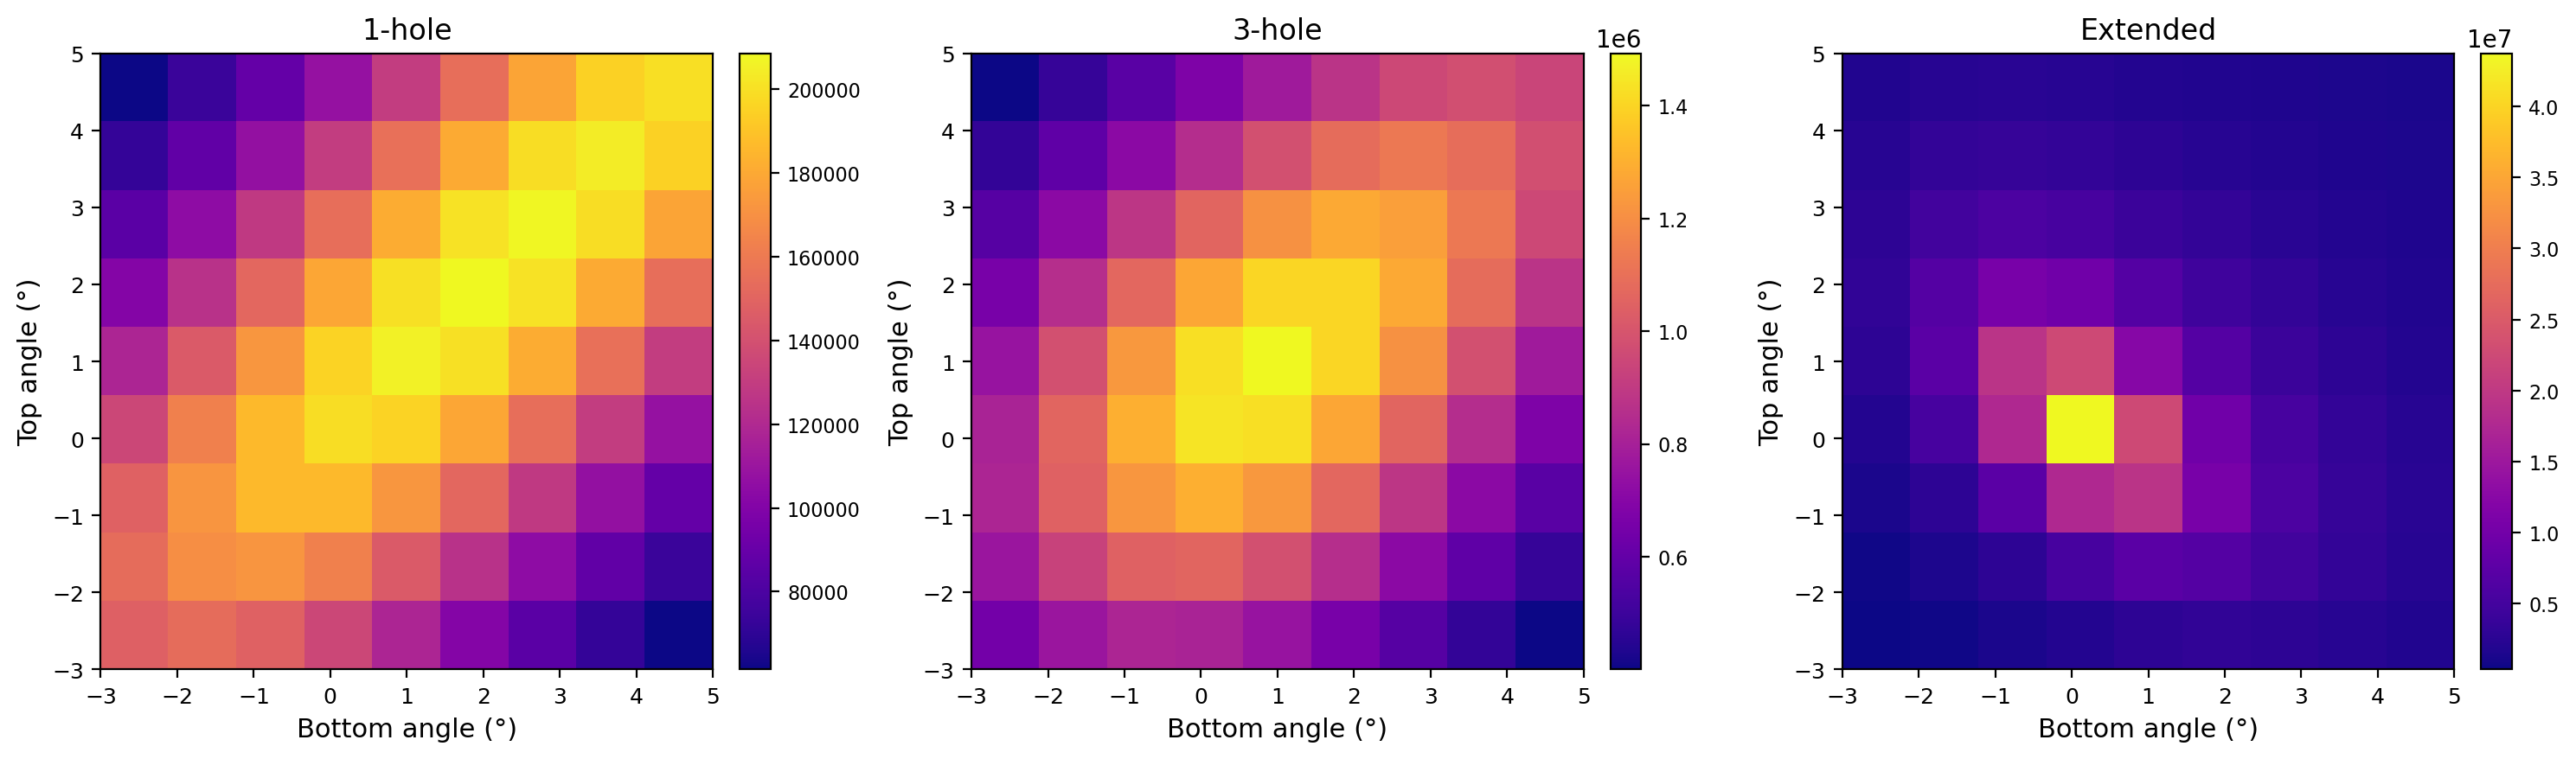
\includegraphics[width=\textwidth]{fig_piecewise_heatmaps.png}
  \caption{Quality factor as a function of independent top and bottom taper angles for the three cavity designs. The color scale differs between panels.}
  \label{fig:piecewise}
\end{figure}


% ----------------------------------------------------------
%  3.4  Q vs. Oxide Thickness (fixed cr)
% ----------------------------------------------------------
\subsection{Quality Factor vs.\ Oxide Thickness (Fixed Consumption Ratio)}
\label{sec:oxide_fixed}

Native oxide growth on GaAs modifies the photonic crystal geometry. We model the oxide as a conformal dielectric layer ($n_\mathrm{ox} = 1.72$) on all hole surfaces and the slab top/bottom. The \emph{consumption ratio}
\begin{equation}
  c_r = \frac{t_\mathrm{consumed\;GaAs}}{t_\mathrm{total\;oxide}}
  \label{eq:cr}
\end{equation}
parameterizes the balance: $c_r = 0$ is pure outward growth (no GaAs removed), $c_r = 1$ is pure inward growth (all oxide replaces GaAs).

Figure~\ref{fig:oxide_fixed_cr} shows $Q$ and $\lambda_0$ vs.\ oxide thickness for the 3-hole design at $c_r = 0.5$ and five radii. At $c_r = 0.5$, the oxide simultaneously increases the effective hole radius (by consuming GaAs) and adds a low-index layer. For $r = \SI{73}{nm}$, which is below the optimum, oxidation initially \emph{improves} $Q$ by shifting the geometry toward the optimum---$Q$ peaks near \SI{4.5}{nm} oxide before declining. For $r = \SI{75}{nm}$ (at optimum), $Q$ decreases monotonically from \num{1438926} to \num{369647} at \SI{10}{nm}---a 74\% reduction. For $r \geq \SI{76}{nm}$, $Q$ drops steeply and exhibits anomalous collapses above \SI{7}{nm} where the mode exits the bandgap.

The wavelength blueshifts at approximately \SI{1.8}{nm} per \si{nm} of oxide, reflecting the replacement of high-index GaAs with low-index oxide.

\begin{figure}[htbp]
  \centering
  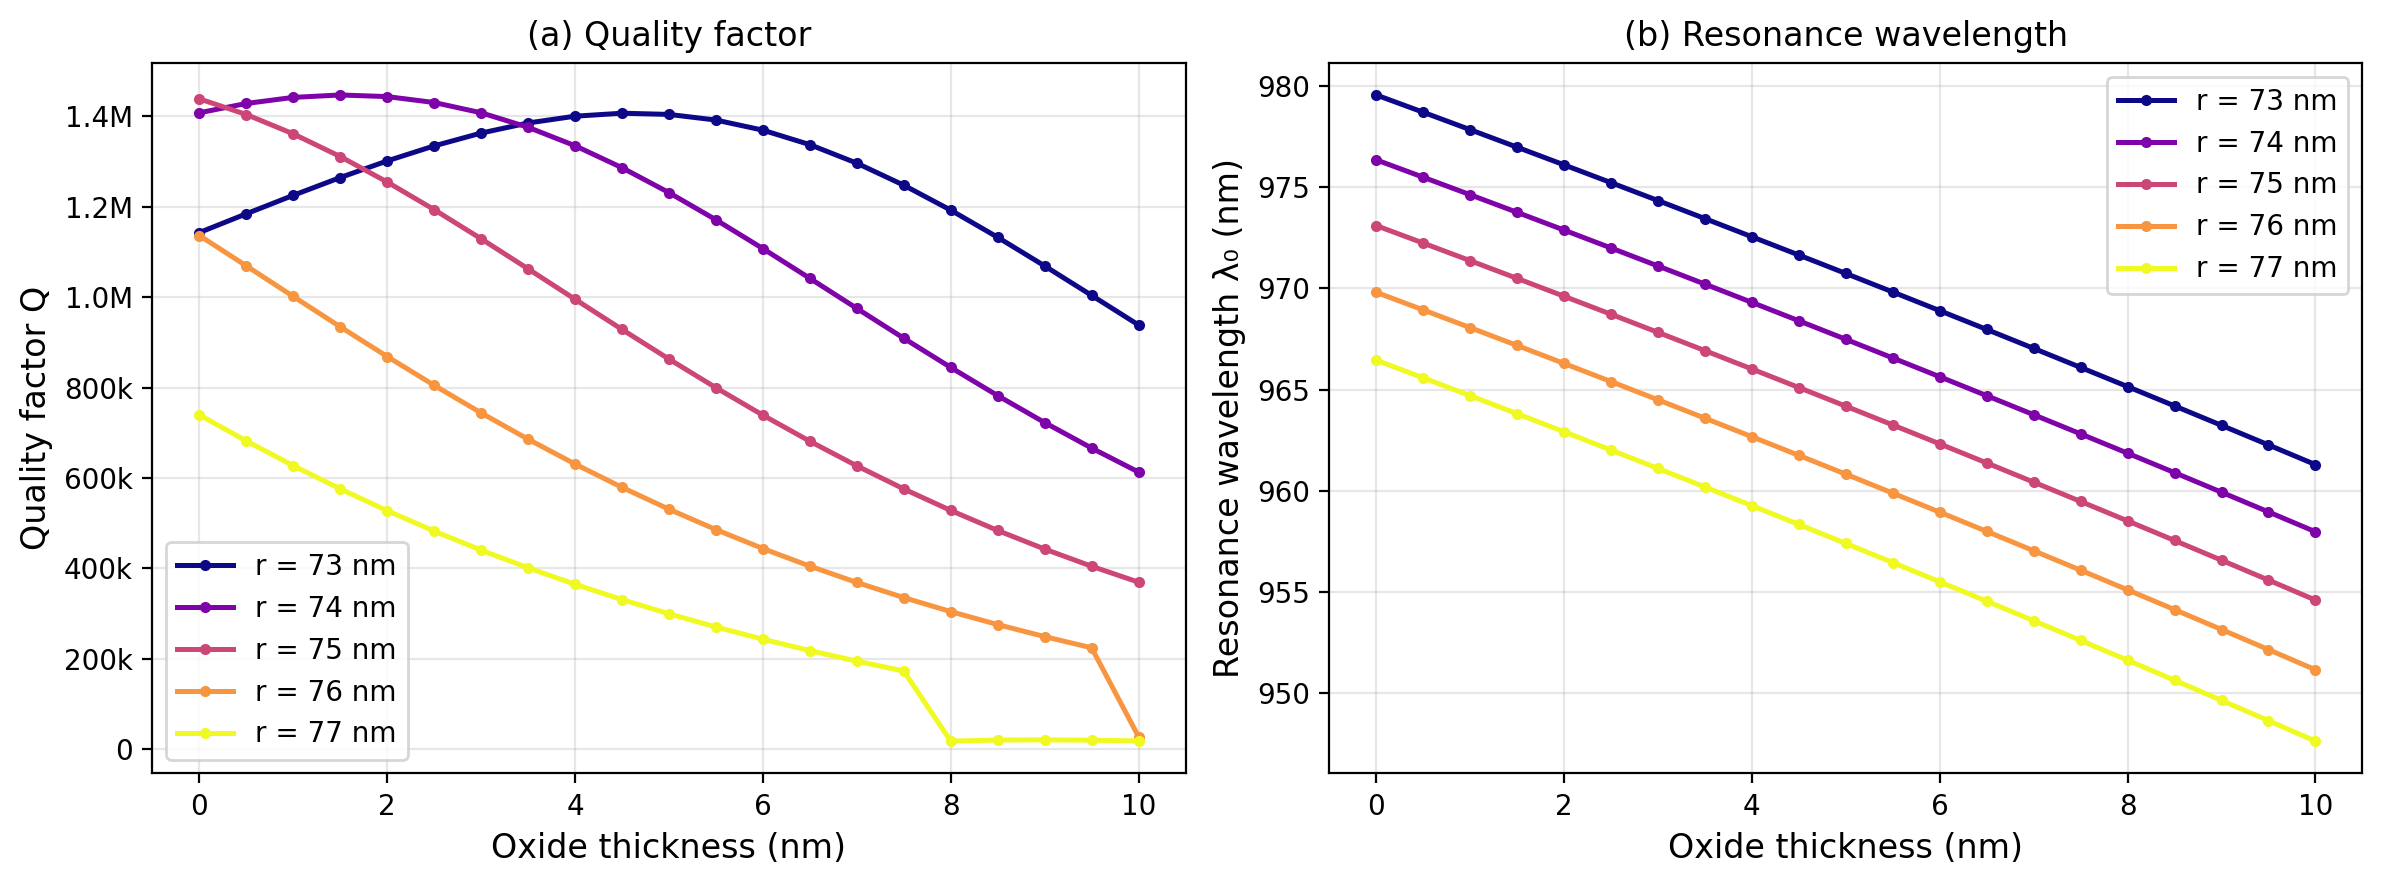
\includegraphics[width=\textwidth]{fig_oxide_fixed_cr.png}
  \caption{Quality factor and resonance wavelength vs.\ oxide thickness for the 3-hole design at $c_r = 0.5$ and five hole radii.}
  \label{fig:oxide_fixed_cr}
\end{figure}

Figure~\ref{fig:oxide_all_designs} compares all three designs at $r = \SI{75}{nm}$ and $c_r = 0.5$. The extended design collapses from \num{43.7e6} to \num{277000} at just \SI{5}{nm} oxide---a factor of 160. \textbf{Fabrication implication:} if the extended design yields any measurable $Q$ at all, the total oxide thickness is likely below \SI{3}{nm}.

\begin{figure}[htbp]
  \centering
  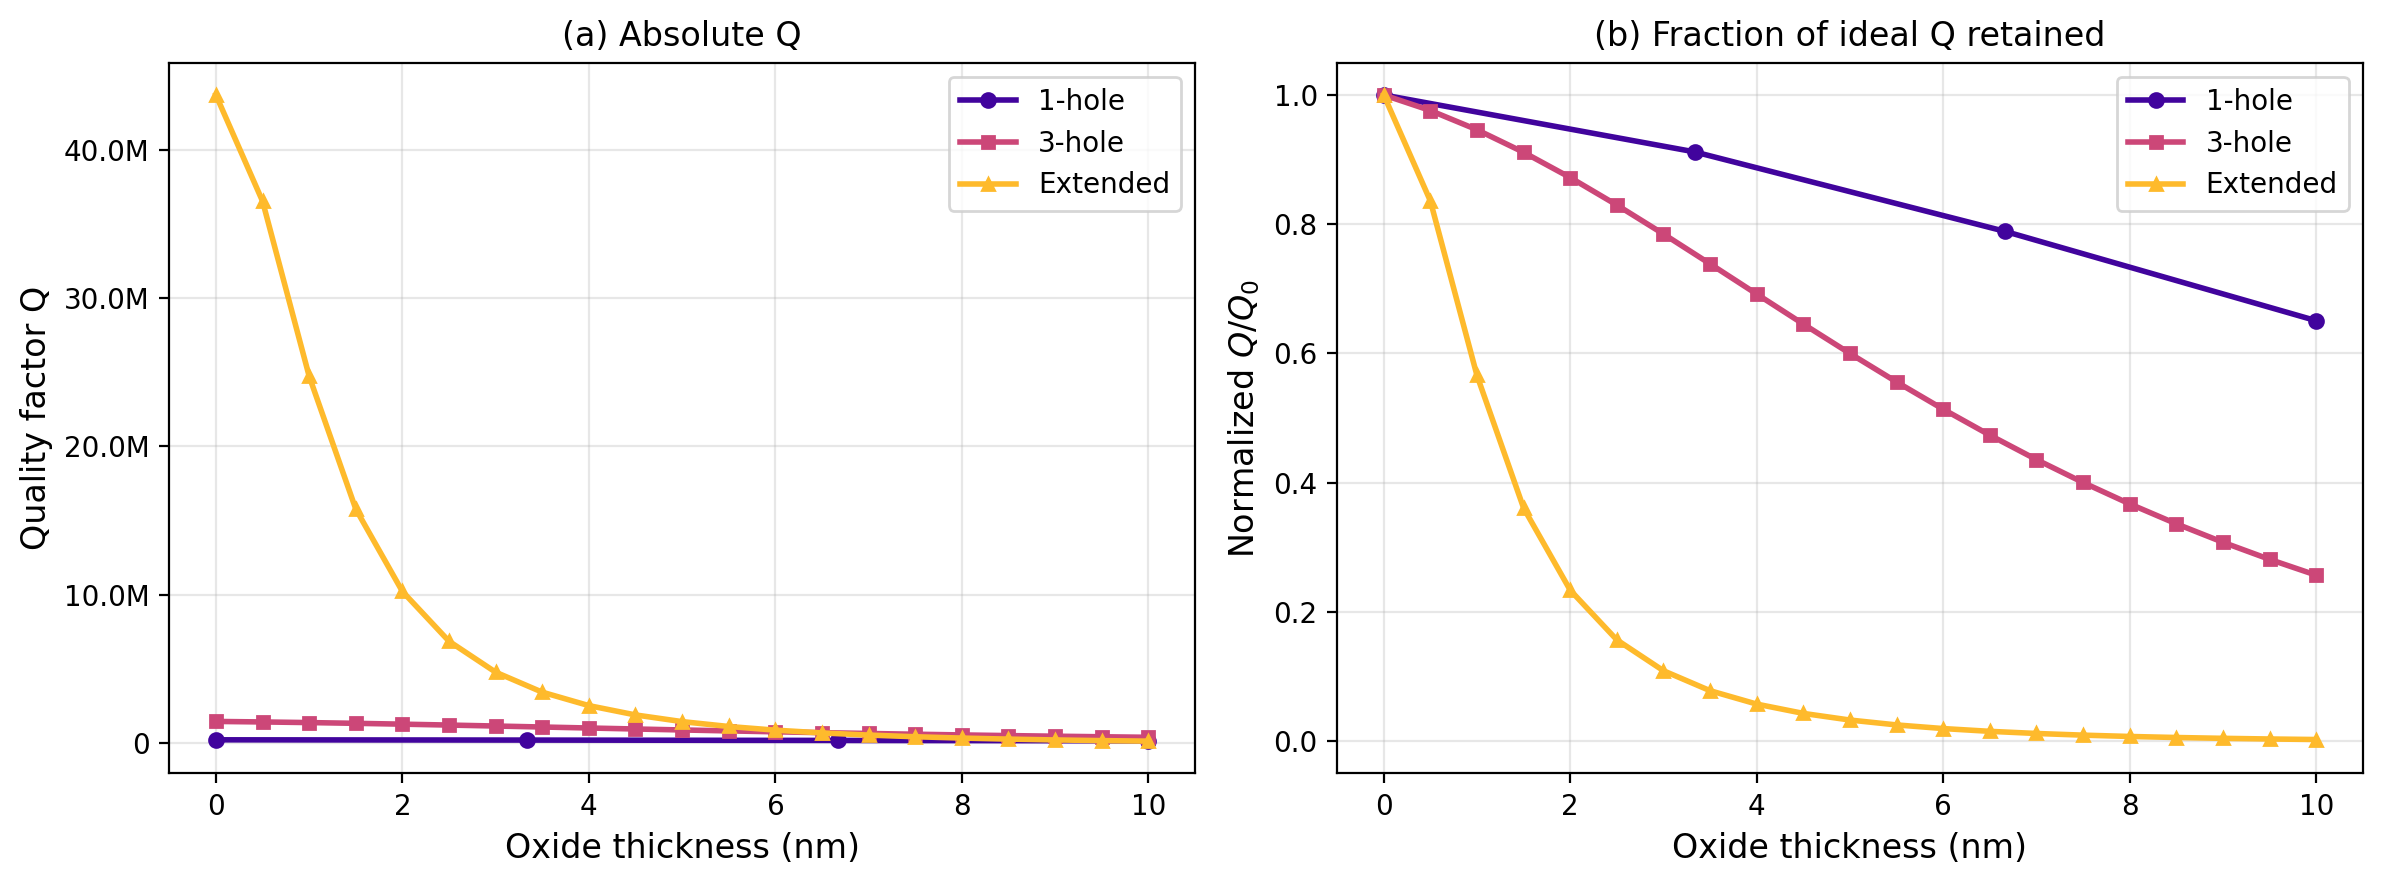
\includegraphics[width=0.7\textwidth]{fig_oxide_all_designs.png}
  \caption{Quality factor vs.\ oxide thickness for all three designs at $r = \SI{75}{nm}$ and $c_r = 0.5$, showing the dramatic sensitivity increase with optimization level.}
  \label{fig:oxide_all_designs}
\end{figure}


% ----------------------------------------------------------
%  3.5  Q vs. Oxide Thickness (varying cr)
% ----------------------------------------------------------
\subsection{Quality Factor vs.\ Oxide Thickness (Varying Consumption Ratio)}
\label{sec:oxide_cr}

The consumption ratio $c_r$ (Eq.~\ref{eq:cr}) is not known \emph{a priori} for our GaAs oxidation process. We therefore sweep $c_r$ from 0.0 to 1.0 at fixed $r = \SI{75}{nm}$ for the 3-hole design (Figure~\ref{fig:oxide_cr}). This is the \textbf{key diagnostic plot} for the characterization chip.

\begin{figure}[htbp]
  \centering
  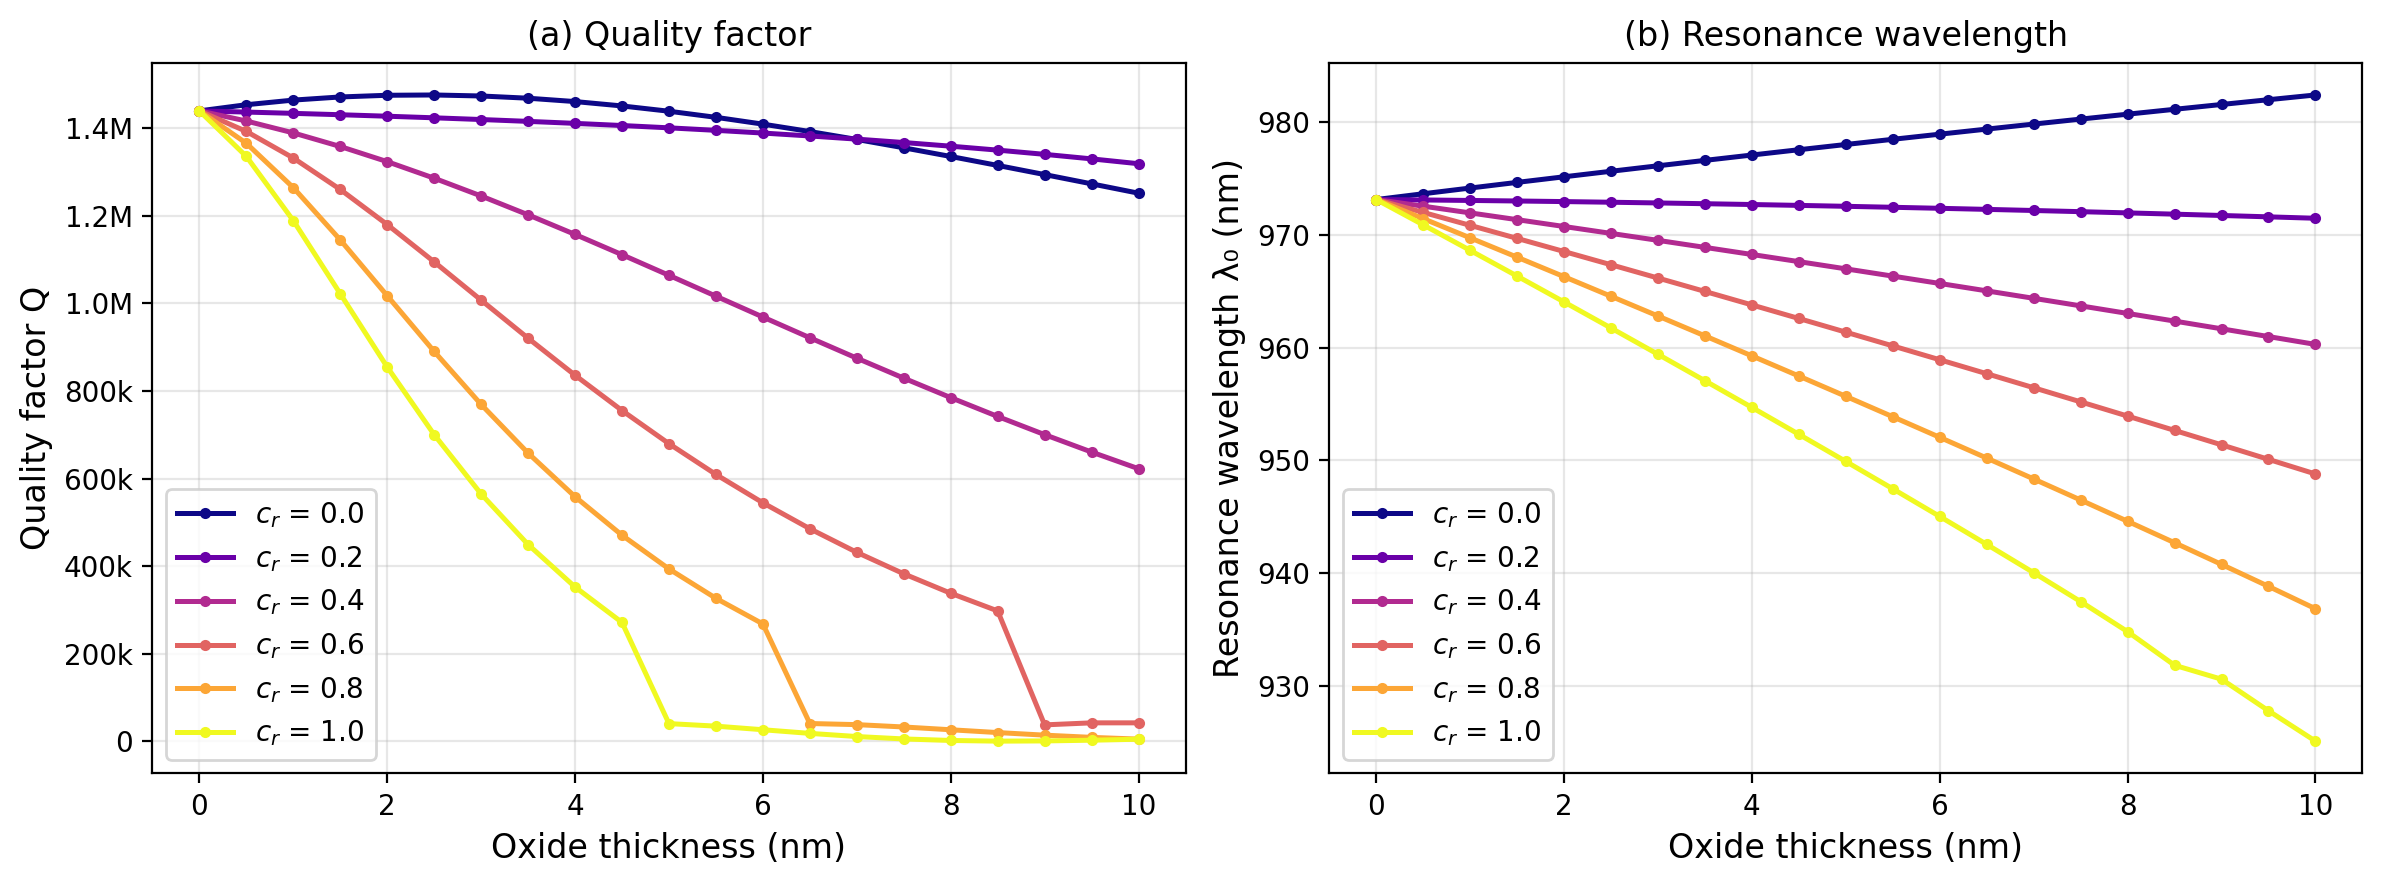
\includegraphics[width=\textwidth]{fig_oxide_varying_cr.png}
  \caption{Quality factor and resonance wavelength vs.\ oxide thickness for the 3-hole design ($r = \SI{75}{nm}$) at six consumption ratios $c_r$. This is the primary diagnostic for extracting $c_r$ from experiment.}
  \label{fig:oxide_cr}
\end{figure}

The results span two qualitatively different regimes:
\begin{itemize}
  \item \textbf{Pure outward growth} ($c_r = 0$): $Q$ \emph{increases slightly} from \num{1438926} to a peak of \num{1475205} near \SI{2.5}{nm} oxide, then decreases gently to \num{1251072} at \SI{10}{nm}---only a 13\% net reduction. The initial improvement arises because the gradual index transition from air through oxide to GaAs acts as an anti-reflection coating on each hole, smoothing the Fourier components of the cavity mode. The wavelength \emph{redshifts} at $\sim$\SI{0.9}{nm}/nm of oxide.
  \item \textbf{Pure consumption} ($c_r = 1$): $Q$ drops catastrophically because the optimized hole geometry is destroyed. At \SI{5}{nm}, $Q$ has already collapsed to \num{40662}. The wavelength \emph{blueshifts} steeply at $\sim$\SI{4.8}{nm}/nm.
  \item \textbf{Intermediate $c_r$}: values interpolate smoothly. $c_r = 0.2$ preserves $Q$ above \num{1.3e6} even at \SI{10}{nm}; $c_r = 0.6$ and 0.8 show sharp collapses at \SIrange{8}{6.5}{nm}.
\end{itemize}

\textbf{Fabrication implication:} the wavelength shift rate depends strongly on $c_r$, from \SI{+0.9}{nm}/nm ($c_r=0$, redshift) to \SI{-4.8}{nm}/nm ($c_r=1$, blueshift). Even a single wavelength measurement before and after controlled oxidation constrains $c_r$. Combined with the $Q$ degradation curve, both $c_r$ and $t_\mathrm{ox}$ can be extracted simultaneously.


% ----------------------------------------------------------
%  3.6  Extended Design Sensitivity
% ----------------------------------------------------------
\subsection{Extended Design: Radius and Oxide Sensitivity}
\label{sec:ext_sensitivity}

The extended design's extreme $Q$ makes it a sensitive probe. Figure~\ref{fig:ext_radius_oxide} shows $Q$ vs.\ oxide thickness at five radii. At $r = \SI{75}{nm}$, $Q$ drops from \num{43.7e6} to \num{109000} at \SI{10}{nm} oxide. Even at $r = \SI{73}{nm}$ (where the 3-hole design showed improvement under oxidation), the extended $Q$ starts at only \num{2.4e6} and never exceeds \num{3.4e6}---far below its optimum, confirming that the extended design is sharply tuned to $r = \SI{75}{nm}$.

\begin{figure}[htbp]
  \centering
  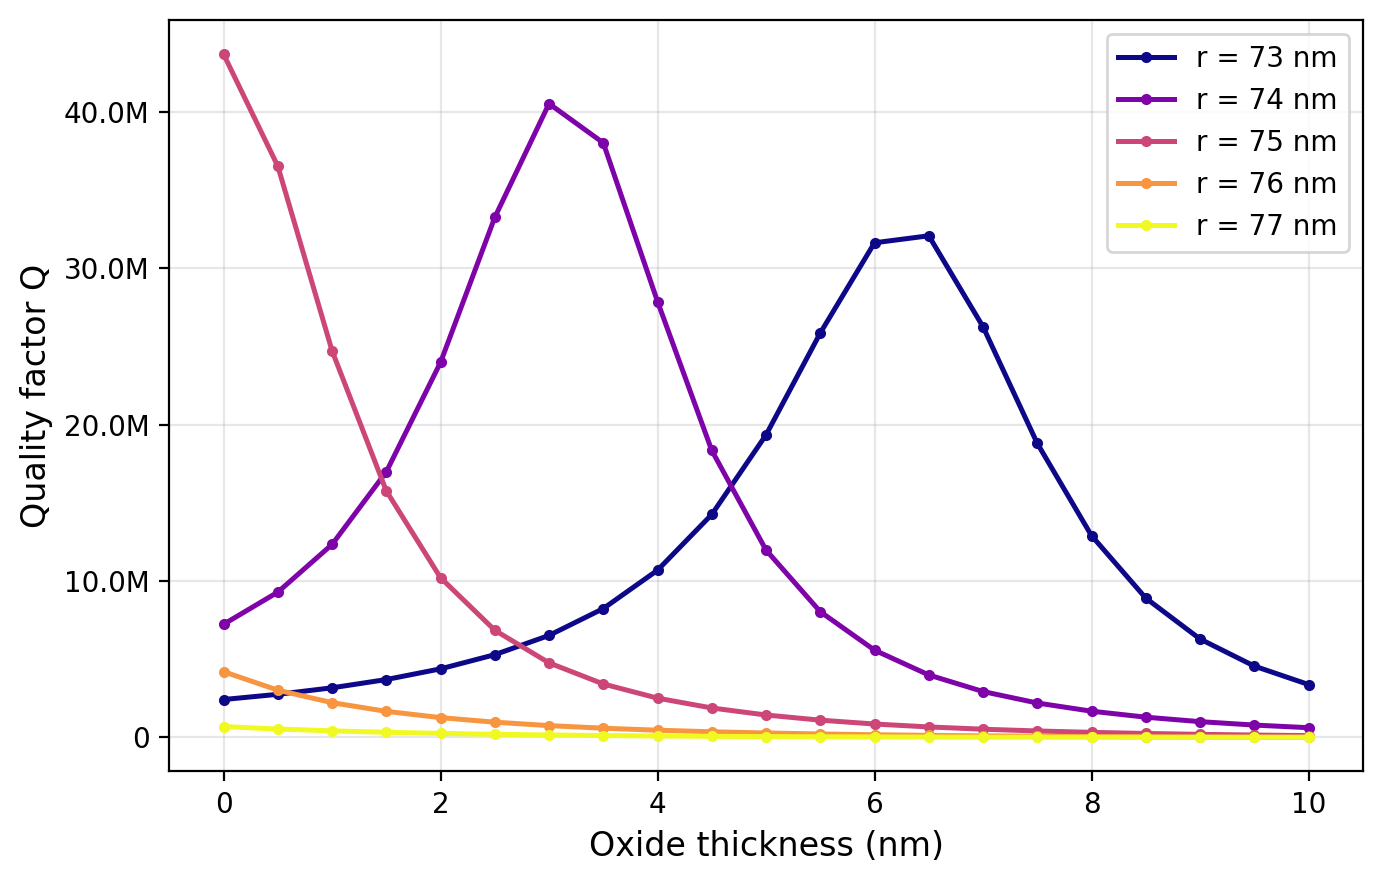
\includegraphics[width=0.7\textwidth]{fig_ext_radius_oxide.png}
  \caption{Quality factor vs.\ oxide thickness for the extended design at five hole radii ($c_r = 0.5$).}
  \label{fig:ext_radius_oxide}
\end{figure}


% ----------------------------------------------------------
%  3.7  Hole Shift Robustness
% ----------------------------------------------------------
\subsection{Sensitivity to Hole Shift ($\mathrm{dx}_1$)}
\label{sec:dx_shift}

In addition to radius and oxide, we investigate how precisely the S1 hole shift must match the design value. Figure~\ref{fig:dx_shift} sweeps $\mathrm{dx}_1$ from $0.160a$ to $0.200a$ (the 1-hole optimum is $0.17964a$) combined with oxide thickness. The $Q$ peak is relatively broad in $\mathrm{dx}_1$, but shifts away from the optimum become compounded by oxidation: at $\mathrm{dx}_1 = 0.16a$, even \SI{3}{nm} of oxide drops $Q$ below \num{100000}.

\textbf{Fabrication implication:} the hole shift tolerance is approximately $\pm 0.01a$ ($\pm\SI{2.5}{nm}$) for the 1-hole design. The 3-hole design would be more sensitive, underscoring the importance of precise e-beam lithography.

\begin{figure}[htbp]
  \centering
  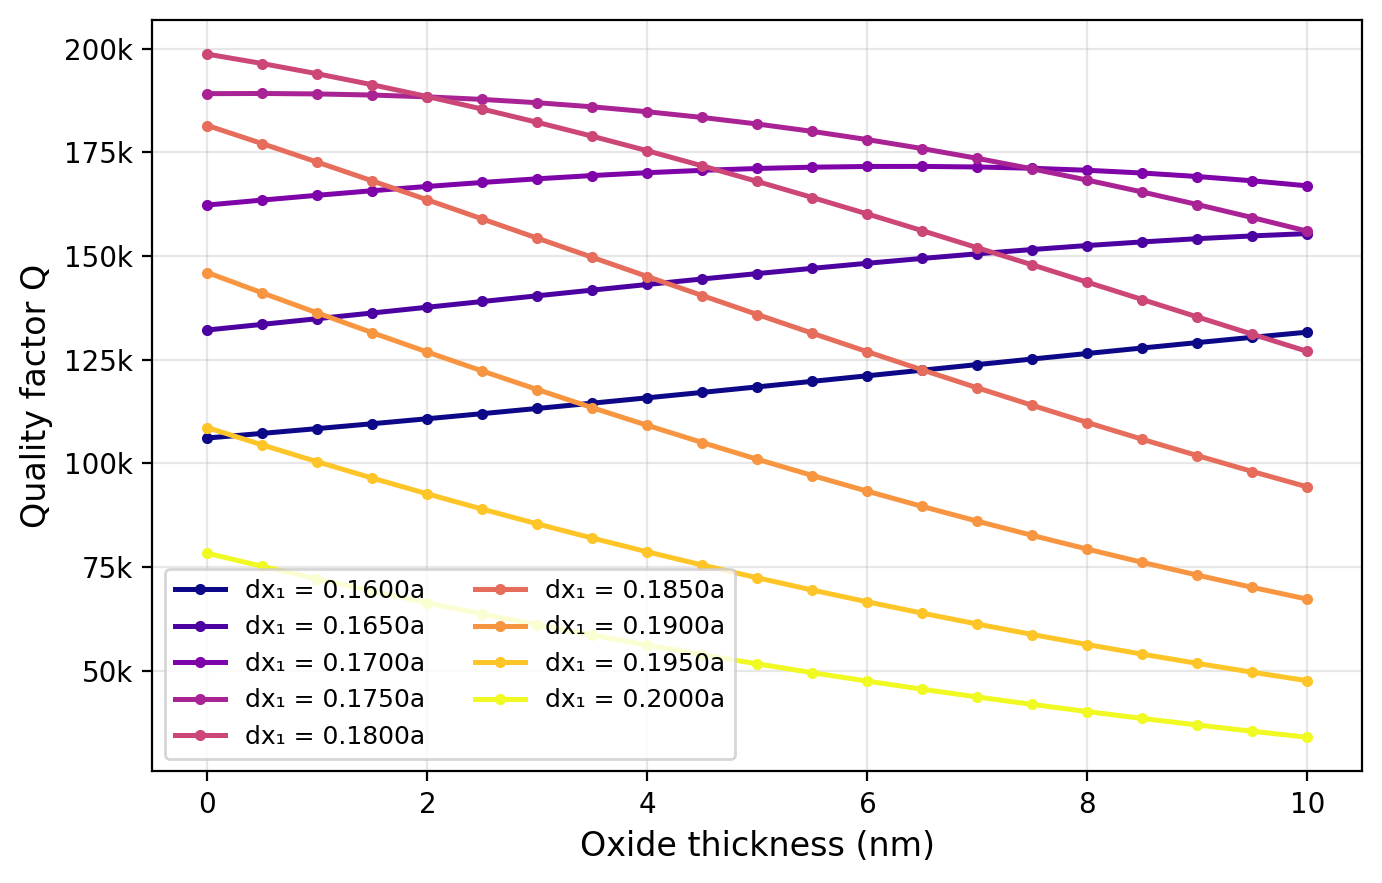
\includegraphics[width=0.7\textwidth]{fig_dx_shift_oxide.png}
  \caption{Quality factor vs.\ oxide thickness for the 1-hole design at nine values of the S1 hole shift $\mathrm{dx}_1$.}
  \label{fig:dx_shift}
\end{figure}


% ----------------------------------------------------------
%  3.8  Conical Taper + Oxide Combined
% ----------------------------------------------------------
\subsection{Combined Taper and Oxide Effects}
\label{sec:conical_oxide}

In practice, taper and oxide are present simultaneously. Figure~\ref{fig:conical_oxide} shows $Q$ vs.\ taper angle at five oxide thicknesses for the 1-hole design. Both imperfections compound: at $\theta = \SI{2}{\degree}$ and $t_\mathrm{ox} = \SI{4}{nm}$, $Q$ has dropped to approximately \num{60000}---less than a third of the ideal value. The wavelength shift from taper (redshift) partially compensates the shift from oxide (blueshift at $c_r > 0$), complicating the extraction of individual contributions from wavelength alone.

\textbf{Fabrication implication:} taper and oxide are not independently measurable from a single device. The row-number sweep and the comparison between optimization levels are needed to decouple them.

\begin{figure}[htbp]
  \centering
  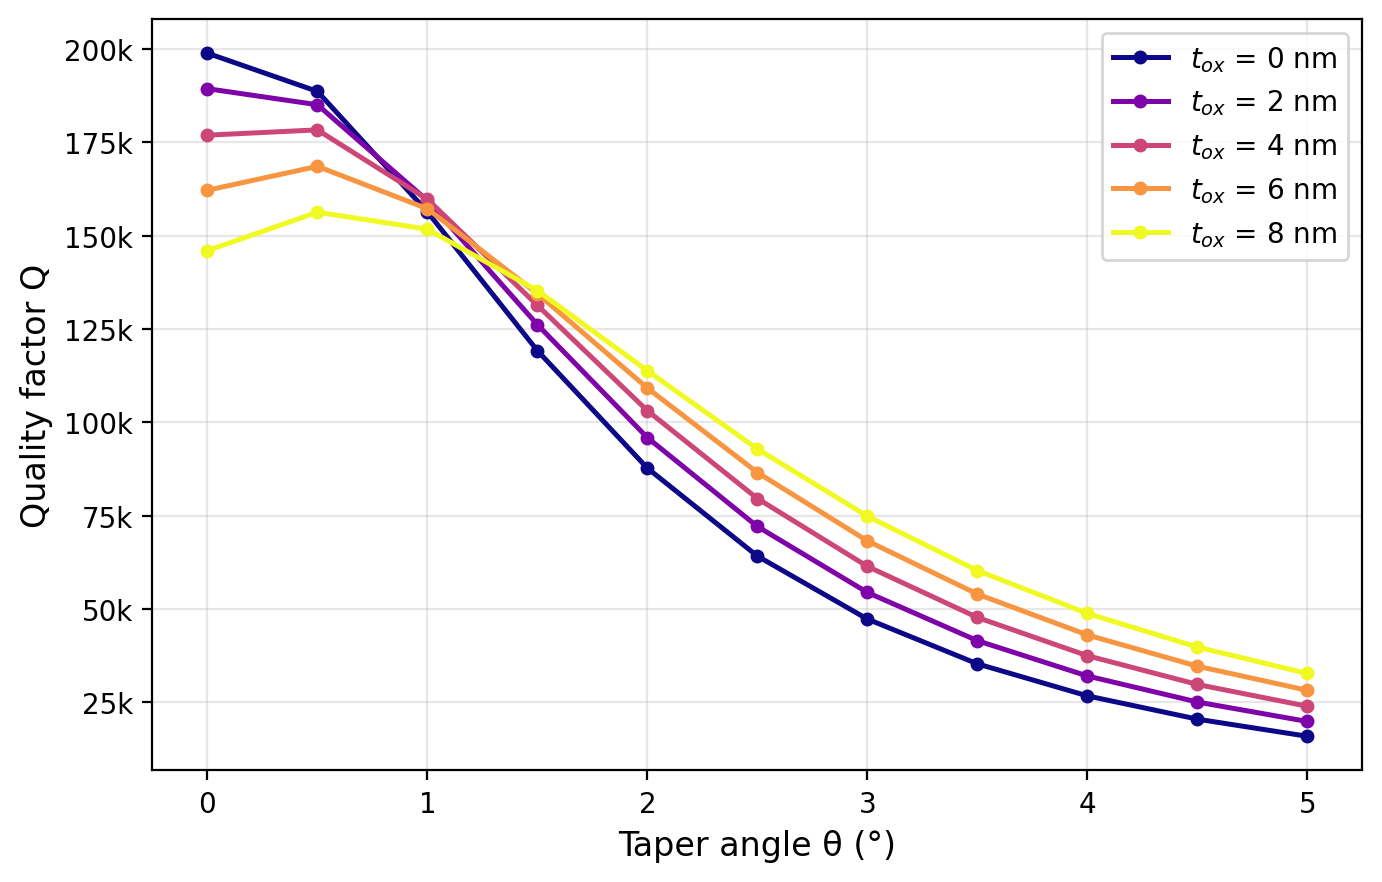
\includegraphics[width=0.7\textwidth]{fig_conical_oxide.png}
  \caption{Quality factor vs.\ taper angle for the 1-hole design at five oxide thicknesses, showing compounding of taper and oxide degradation.}
  \label{fig:conical_oxide}
\end{figure}


% ----------------------------------------------------------
%  3.9  Ellipticity
% ----------------------------------------------------------
\subsection{Hole Ellipticity and Rotation}
\label{sec:ellipticity}

Fabrication may produce slightly elliptical holes rather than perfect circles. We parameterize hole shape by an ellipticity $e = r_y / r_x$, where $e = 1$ is circular. Figure~\ref{fig:ellipticity} compares all three designs.

The 1-hole design shows an asymmetric response: $Q$ increases for $e > 1$ (holes elongated perpendicular to the cavity axis), reaching \num{204000} at $e = 1.6$, while dropping sharply for $e < 1$. The 3-hole design shows a similar asymmetry but with a narrower peak. The extended design peaks sharply at $e = 1.0$ and collapses in both directions.

Figure~\ref{fig:ellipticity_rotation} shows 2D heatmaps of $Q$ vs.\ ellipticity and rotation angle. For the 1-hole design, the optimal region extends broadly toward high ellipticity at $0^\circ$ rotation, suggesting that mild elongation perpendicular to the cavity axis may actually be beneficial. For the extended design, the optimum is a single narrow peak at $e = 1.0$.

\begin{figure}[htbp]
  \centering
  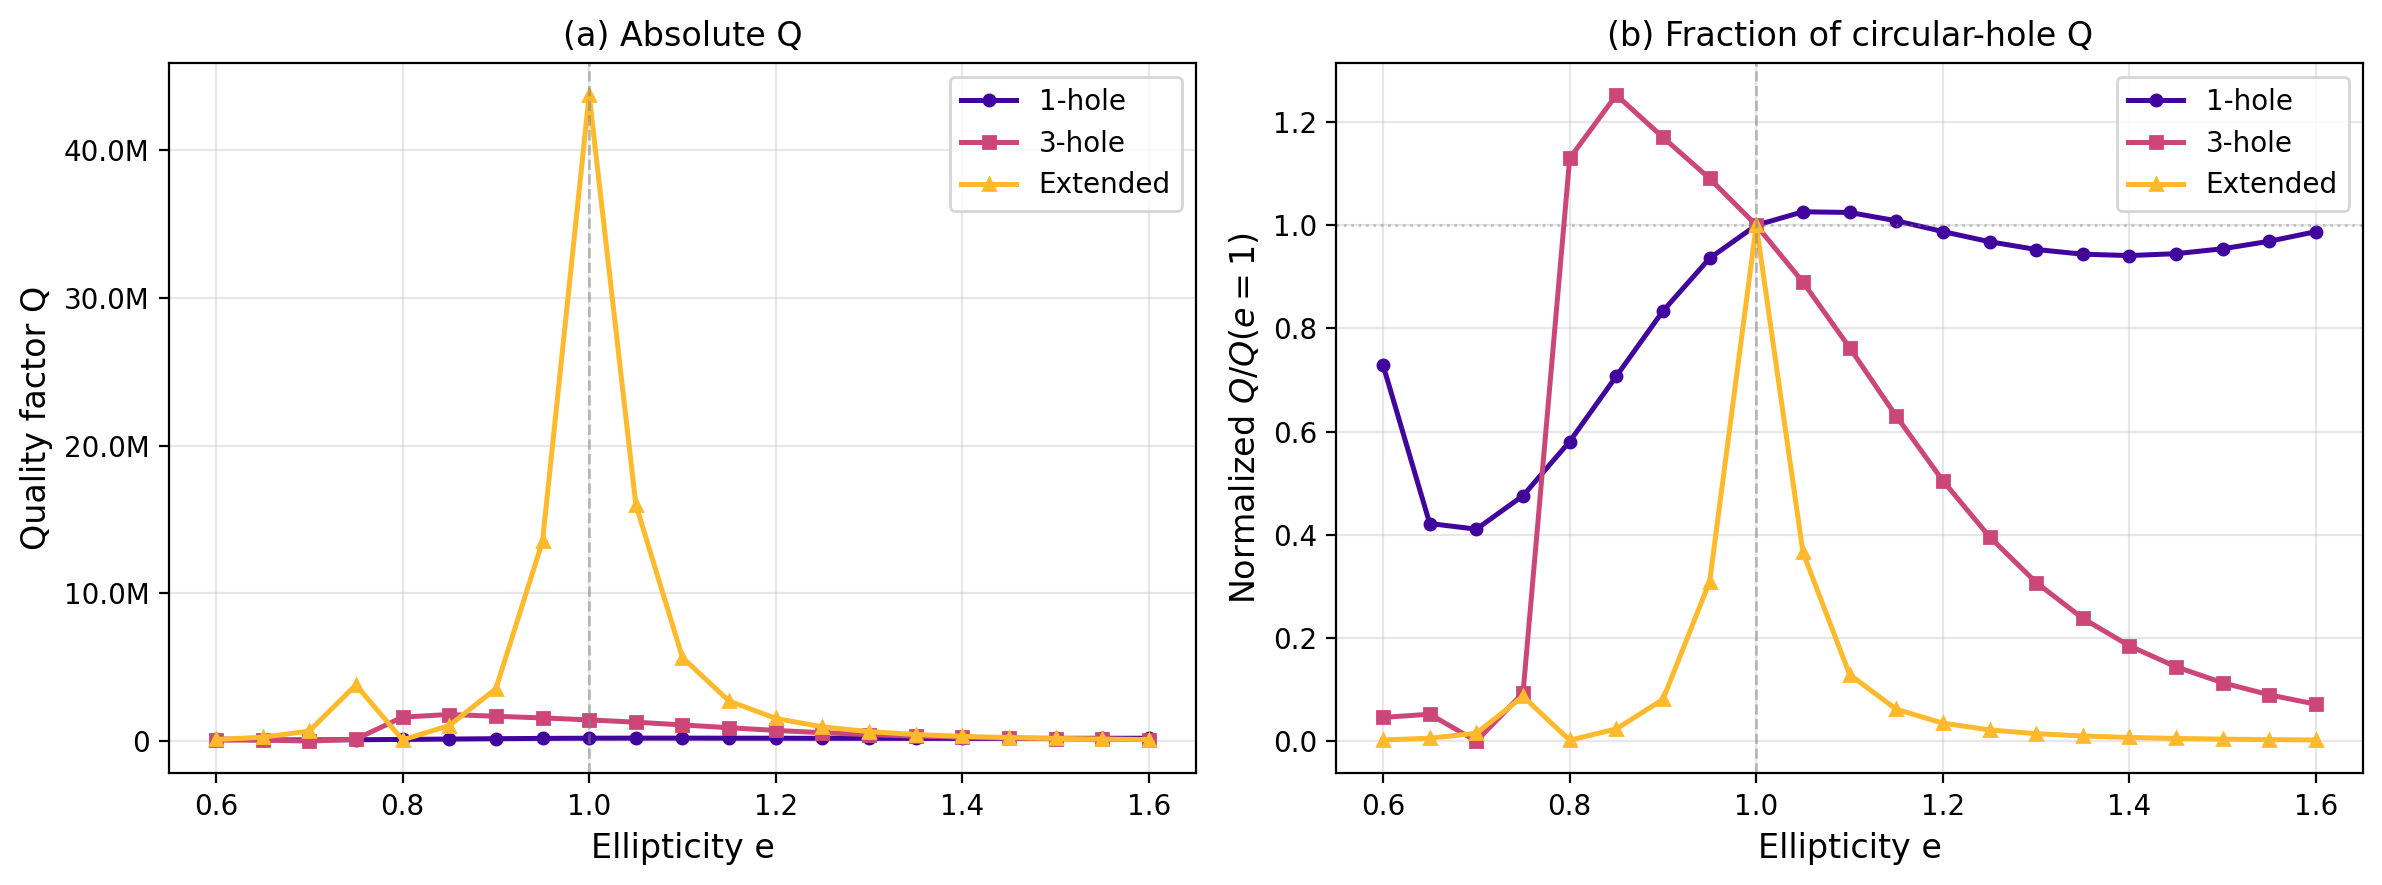
\includegraphics[width=0.7\textwidth]{fig_ellipticity_combined.png}
  \caption{Quality factor vs.\ hole ellipticity for all three designs. The dashed line marks circular holes ($e = 1$).}
  \label{fig:ellipticity}
\end{figure}

\begin{figure}[htbp]
  \centering
  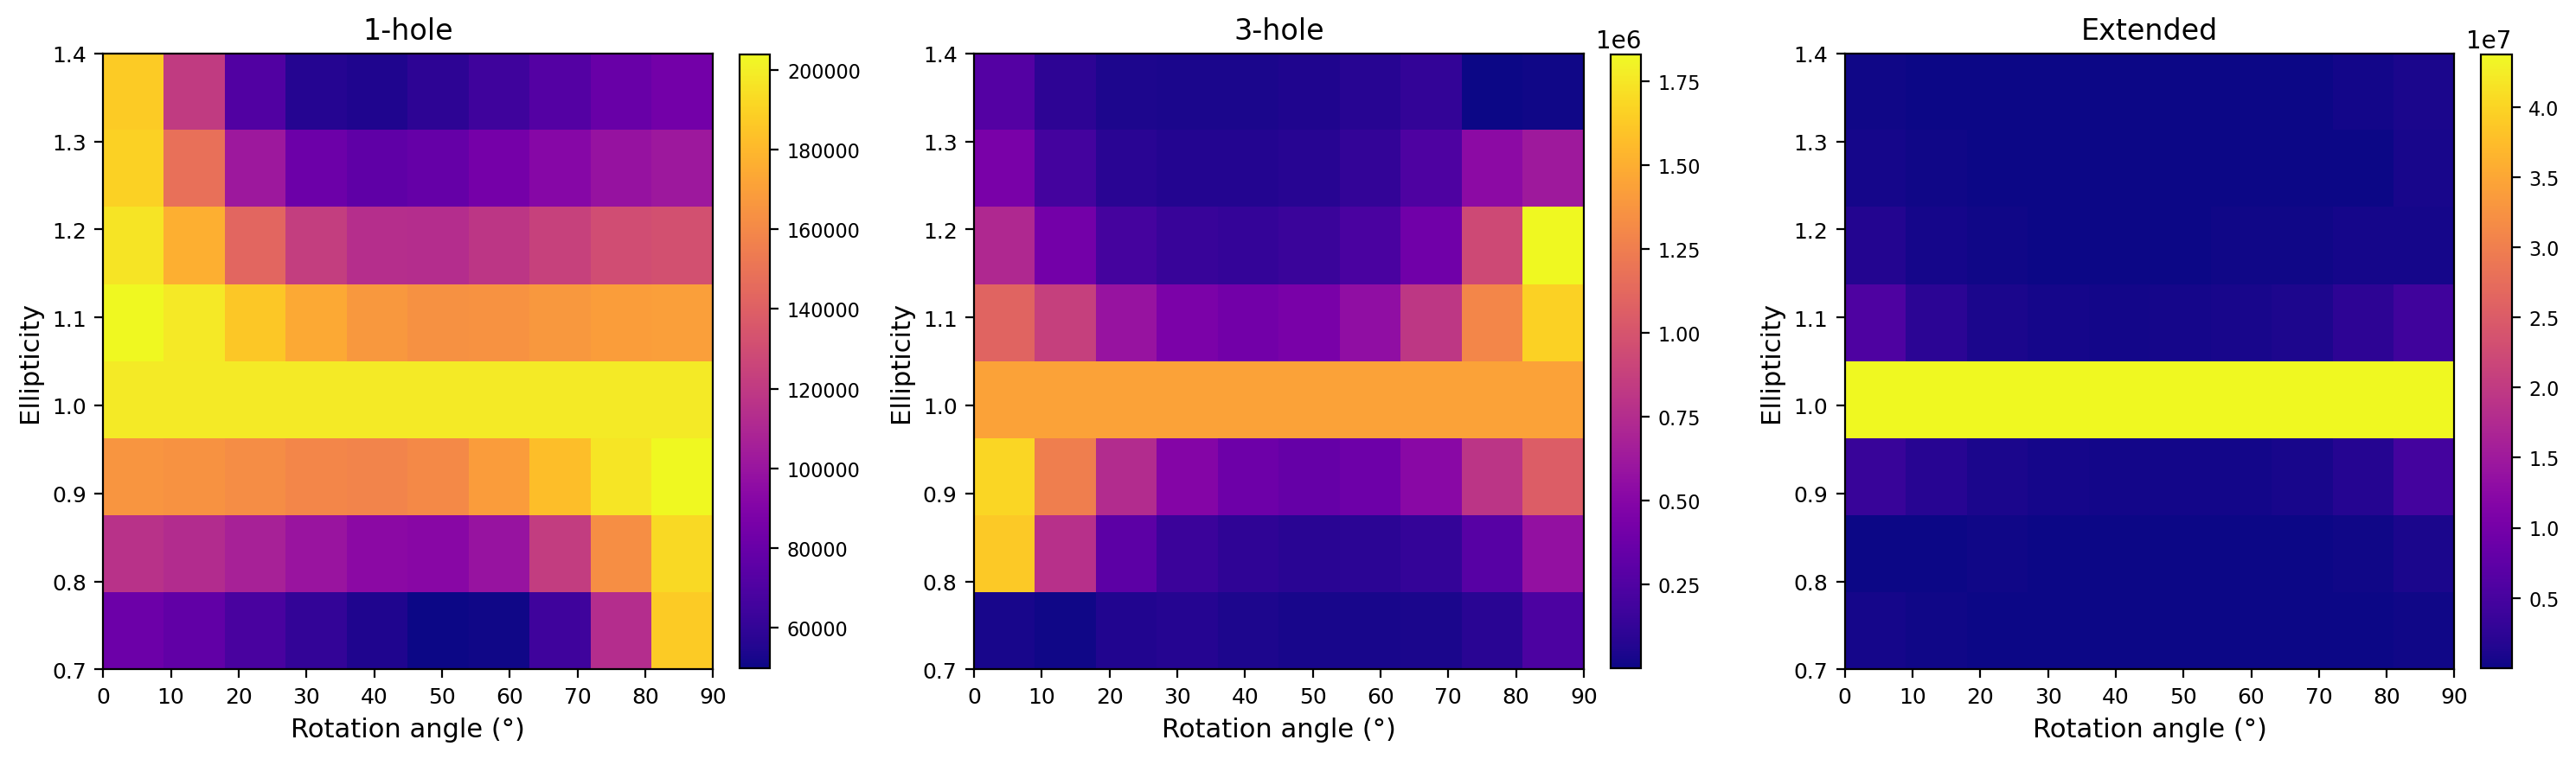
\includegraphics[width=\textwidth]{fig_ellipticity_rotation.png}
  \caption{Quality factor as a function of ellipticity and rotation angle for the three designs. Color scales differ between panels.}
  \label{fig:ellipticity_rotation}
\end{figure}


% ----------------------------------------------------------
%  3.10  Random Oxide Variation
% ----------------------------------------------------------
\subsection{Random Oxide Thickness Variation}
\label{sec:random_oxide}

To assess robustness to non-uniform oxide growth, we add Gaussian-distributed random variations to the oxide thickness on each hole with standard deviation $\sigma$. Figure~\ref{fig:random_oxide}a shows $Q$ vs.\ $\sigma$ for the 1-hole design (10 random realizations per point). $Q$ degrades gracefully: at $\sigma = \SI{0.3}{nm}$, the mean $Q$ is still $\sim$\num{170000} (86\% of ideal), and even at $\sigma = \SI{0.5}{nm}$ it remains $\sim$\num{155000}.

Figure~\ref{fig:random_oxide}b shows the combined effect of mean oxide thickness and random variation. At zero mean oxide, randomness alone has only a modest effect. As mean oxide increases, randomness amplifies the degradation because the cavity is already operating away from its optimal geometry.

\textbf{Fabrication implication:} the 1-hole design is robust to oxide thickness non-uniformity at the sub-nanometer level typical of native oxides. The 3-hole design would be less tolerant.

\begin{figure}[htbp]
  \centering
  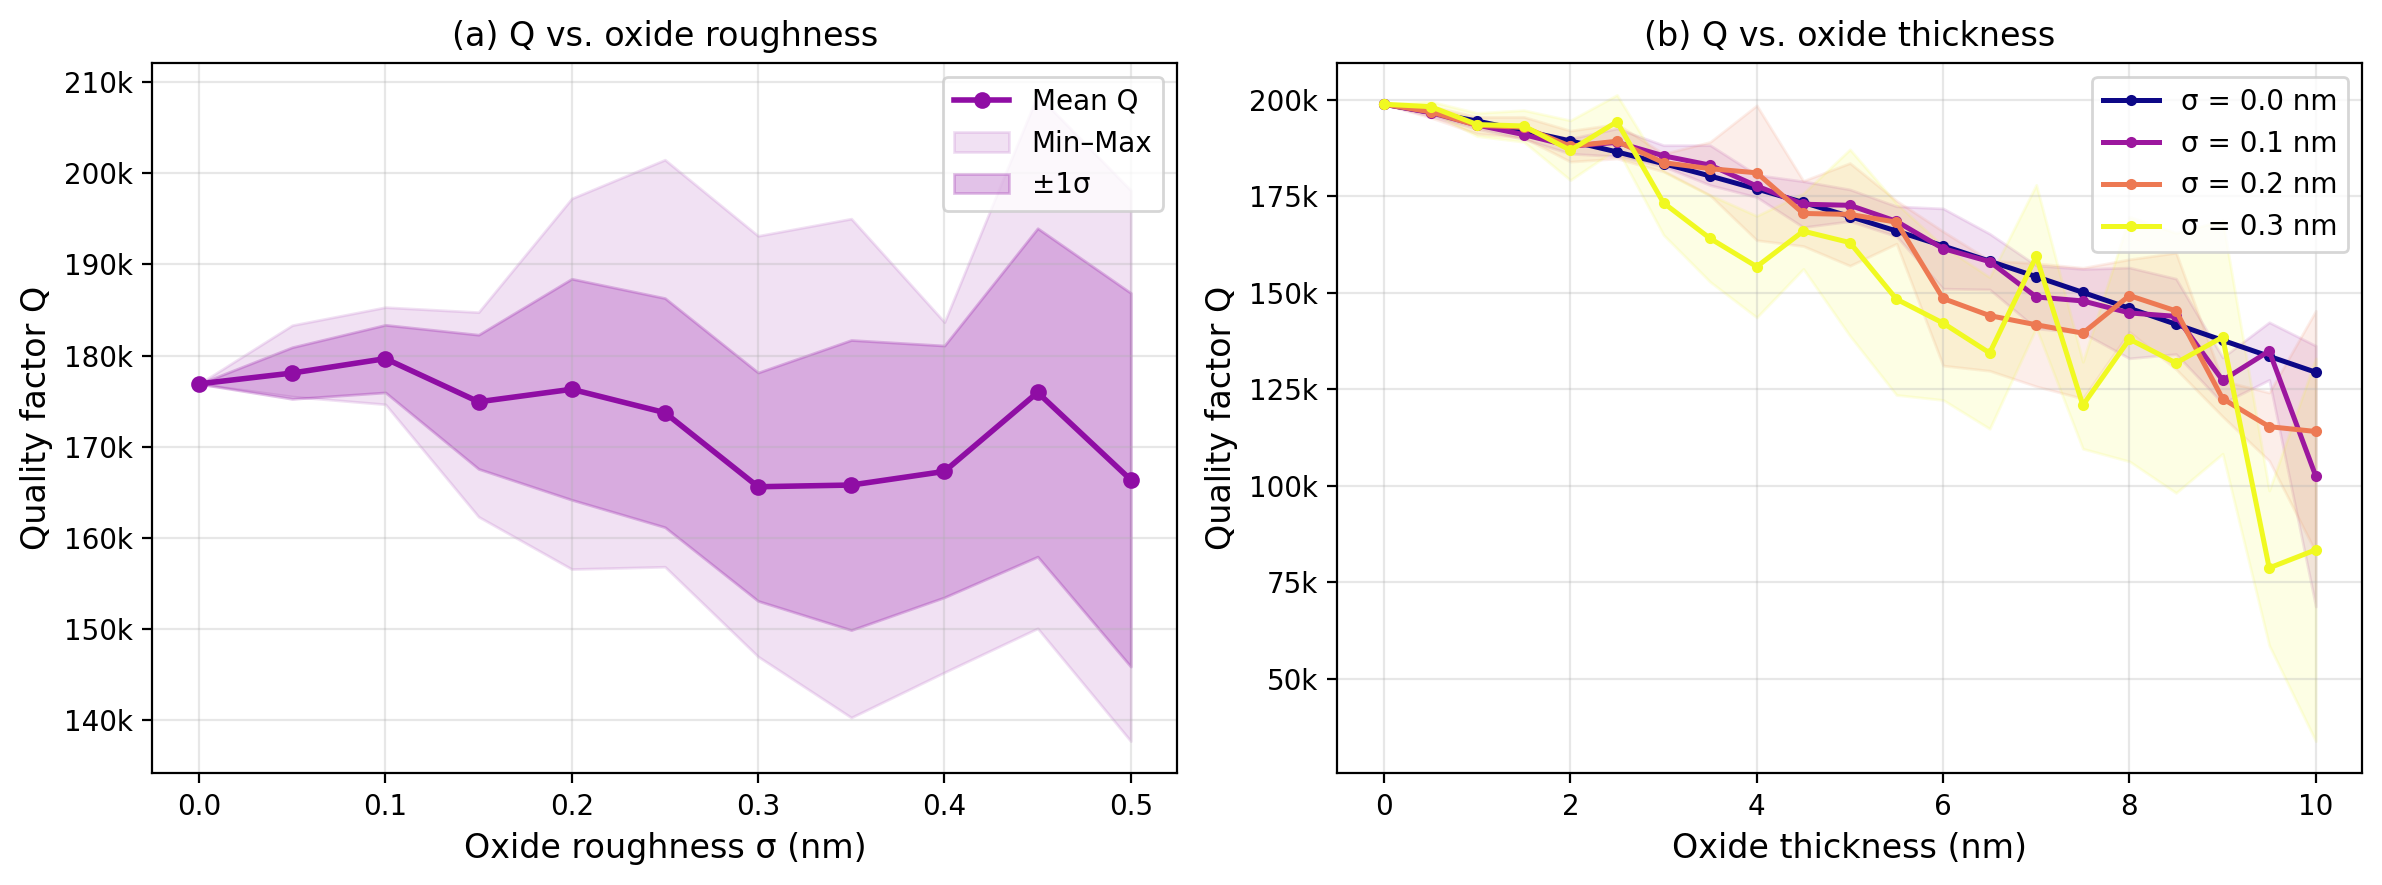
\includegraphics[width=\textwidth]{fig_random_oxide.png}
  \caption{Effect of random oxide thickness variation on the 1-hole design. (a)~$Q$ vs.\ roughness $\sigma$ at fixed mean oxide. (b)~$Q$ vs.\ mean oxide thickness at four levels of randomness. Shaded bands show $\pm 1\sigma$ across realizations.}
  \label{fig:random_oxide}
\end{figure}


% ----------------------------------------------------------
%  3.11  Q vs. Number of PhC Rows
% ----------------------------------------------------------
\subsection{Quality Factor vs.\ Number of PhC Rows}
\label{sec:rows}

The total quality factor of a PhC cavity decomposes as
\begin{equation}
  \frac{1}{Q_\mathrm{total}} = \frac{1}{Q_\perp} + \frac{1}{Q_\parallel(d)}
  \label{eq:Q_decomposition}
\end{equation}
where $Q_\perp$ is the out-of-plane (vertical) quality factor and $Q_\parallel(d)$ is the in-plane quality factor due to leakage through $d$ rows of PhC mirror. Because the bandgap provides exponential attenuation, $Q_\parallel(d)$ grows exponentially with $d$ and rapidly saturates the total $Q$ at $Q_\perp$.

On the characterization chip, a row-number sweep ($d = 7$--$12$) will measure this saturation curve. The saturation level gives $Q_\perp$ directly, while the approach rate reveals the in-plane attenuation length. This is crucial because taper primarily degrades $Q_\perp$ while disorder affects both.

\emph{Note:} The simulations in this report use a fixed supercell of $N_y = 10$ rows. A dedicated row-number sweep is planned and will be added to a future revision.


% ----------------------------------------------------------
%  3.12  Lattice Constant (Validation)
% ----------------------------------------------------------
\subsection{Lattice Constant Sweep (Validation)}
\label{sec:lattice}

As a validation of the simulation framework, we sweep $a$ from \SI{220}{nm} to \SI{280}{nm} while keeping $r/a$ and $d/a$ fixed. Maxwell's equations are scale-invariant, so $Q$ should remain constant while $\lambda_0$ scales linearly. The simulation confirms this exactly: $Q = \num{1438926}$ for all 13 values of $a$, and $\lambda_0$ scales from \SI{856}{nm} to \SI{1090}{nm}. This validates the GME implementation and confirms that any experimental $Q(a)$ variation at fixed $r/a$ must arise from fabrication effects.


%% ============================================================
%%  4. IMPLICATIONS FOR CHIP DESIGN
%% ============================================================
\section{Implications for Chip Design}
\label{sec:chip}

The simulation results establish a framework for interpreting experimental data from the characterization chip. Each fabrication imperfection produces a distinct signature in the observables ($Q$, $\lambda_0$, and their dependence on design parameters), enabling a differential diagnosis.

\subsection{Diagnostic Signatures}
\label{sec:signatures}

Table~\ref{tab:signatures} summarizes how each imperfection affects the key observables. The critical insight is that no single observable isolates a single imperfection---it is the \emph{combination} of multiple sweeps and design comparisons that enables separation.

\begin{table}[htbp]
  \centering
  \caption{Diagnostic signatures of fabrication imperfections.}
  \label{tab:signatures}
  \begin{tabular}{@{}lcccc@{}}
    \toprule
    Imperfection & $Q$ reduction & $\lambda_0$ shift & Design dependence & Row dependence \\
    \midrule
    Radius error & Moderate & Linear & Sharper for 3-hole & Weak \\
    Sidewall taper & Severe & Redshift & All converge at large $\theta$ & Affects $Q_\perp$ only \\
    Oxide ($c_r > 0$) & Moderate--severe & Blueshift & Sharper for 3-hole & Weak \\
    Oxide ($c_r = 0$) & Mild improvement & Redshift & Mild for all & None \\
    Positional disorder & Moderate & Random & Sharper for 3-hole & Affects both \\
    Ellipticity & Mild (if $e > 1$) & Small & 1-hole tolerant & Weak \\
    \bottomrule
  \end{tabular}
\end{table}

\subsection{Measurement Strategy}
\label{sec:strategy}

The characterization chip implements the following diagnostic elements:

\begin{enumerate}
  \item \textbf{Radius sweep} ($r = \SIrange{73}{77}{nm}$): Maps the experimental $Q(r)$ and $\lambda_0(r)$ curves. The wavelength serves as an ``oxidation ruler''---comparing the measured $\lambda_0$ shift against the simulation curves of Figures~\ref{fig:oxide_fixed_cr} and~\ref{fig:oxide_cr} constrains $t_\mathrm{ox}$ and $c_r$ simultaneously.

  \item \textbf{Row-number sweep} ($d = 7$--$12$): Measures the $Q(d)$ saturation to extract $Q_\perp$ and $Q_\parallel$ via Eq.~\ref{eq:Q_decomposition}. If $Q_\perp$ is substantially below the simulated value, taper is the dominant degradation. If $Q_\parallel$ saturates slowly, in-plane disorder is significant.

  \item \textbf{Paired 1-hole and 3-hole designs} at each $(r, d)$: The ratio $Q_\mathrm{3h}/Q_\mathrm{1h}$ is the most powerful single diagnostic:
  \begin{itemize}
    \item If $Q_\mathrm{3h}/Q_\mathrm{1h} \approx 7$ (the simulated ratio): fabrication is nearly ideal.
    \item If $Q_\mathrm{3h}/Q_\mathrm{1h} \approx 1$--$2$: large disorder or taper dominates (both designs are in the disorder-limited regime).
    \item If $Q_\mathrm{3h}/Q_\mathrm{1h} \approx 3$--$5$: moderate disorder with the 3-hole design partially sensitive to design $Q$.
  \end{itemize}

  \item \textbf{Extended design} at $r = 74$, $75$, \SI{76}{nm}: If $Q_\mathrm{ext} > 10^5$, fabrication disorder is very low ($\sigma_r < \SI{0.5}{nm}$); if $Q_\mathrm{ext} < 10^4$, significant geometric imperfections are present (Figure~\ref{fig:ext_radius_oxide}).

  \item \textbf{Two identical chips} from the same wafer: one passivated immediately, one left bare. Periodic re-measurement of the bare chip tracks native oxide growth via the wavelength blueshift. By comparing against Figure~\ref{fig:oxide_cr}, both $c_r$ and $t_\mathrm{ox}(t)$ can be extracted as functions of time.
\end{enumerate}

\subsection{Proposed Chip Layout}

Table~\ref{tab:chip} summarizes the proposed layout.

\begin{table}[htbp]
  \centering
  \caption{Proposed characterization chip layout.}
  \label{tab:chip}
  \begin{tabular}{@{}llll@{}}
    \toprule
    Feature & Design(s) & Varied parameter & Purpose \\
    \midrule
    Radius sweep  & 1-hole + 3-hole & $r = 73$--\SI{77}{nm} & Map $Q(r)$; oxidation ruler \\
    Row sweep     & 1-hole + 3-hole & $d = 7$--$12$ rows & Decouple $Q_\perp$ vs.\ $Q_\parallel$ \\
    Extended      & Extended        & $r = 74, 75, \SI{76}{nm}$ & Sensitivity canary \\
    Passivation   & All             & Passivated vs.\ bare & Track oxide growth \\
    \bottomrule
  \end{tabular}
\end{table}

\subsection{Extracting Parameters from Measurement}
\label{sec:extraction}

Given an experimental dataset of $Q$ and $\lambda_0$ for all designs, the extraction procedure is:
\begin{enumerate}
  \item \textbf{Determine $r_\mathrm{fab}$} from the bare-chip $\lambda_0$ using the radius--wavelength calibration (Figure~\ref{fig:Q_vs_r}b).
  \item \textbf{Determine $t_\mathrm{ox}$ and $c_r$} from the wavelength shift between passivated and bare chips, using the consume-ratio curves (Figure~\ref{fig:oxide_cr}b).
  \item \textbf{Determine taper $\theta$} from the $Q_\perp$ extracted by the row-number sweep, compared against the taper simulation (Figure~\ref{fig:Q_vs_taper_all}).
  \item \textbf{Assess residual disorder} from the remaining discrepancy between simulated and measured $Q$ after accounting for oxide and taper.
  \item \textbf{Cross-check} with the $Q_\mathrm{3h}/Q_\mathrm{1h}$ ratio and the extended-design $Q$ to confirm consistency.
\end{enumerate}


%% ============================================================
%%  5. CONCLUSION
%% ============================================================
\section{Conclusion}
\label{sec:conclusion}

We have presented a comprehensive set of guided-mode expansion simulations for GaAs air-bridge L3 photonic crystal cavities at three optimization levels. The key findings are:

\begin{itemize}
  \item The 3-hole globally optimized design achieves $Q = \num{1438926}$, a $7.2\times$ improvement over the 1-hole design ($Q = \num{198852}$), at the cost of sharper sensitivity to fabrication errors.

  \item Sidewall taper is the most severe single degradation mechanism: \SI{1}{\degree} of taper reduces $Q$ by 21--92\% depending on the optimization level. All designs converge at large taper angles.

  \item Native oxide effects depend critically on the consumption ratio $c_r$. Pure outward growth ($c_r = 0$) is benign and can slightly improve $Q$ via index smoothing, while pure consumption ($c_r = 1$) destroys the cavity. The wavelength shift rate provides an independent handle on $c_r$.

  \item Hole ellipticity with $e > 1$ (elongation perpendicular to the cavity axis) can modestly improve $Q$ for the 1-hole design, providing an unexpected fabrication tolerance. The extended design is intolerant of any ellipticity.

  \item The extended optimization ($Q = \num{43715163}$) serves as a fabrication quality canary: its rapid $Q$ collapse under any perturbation makes it the most sensitive probe available.

  \item Random oxide thickness variations at the sub-nanometer level ($\sigma < \SI{0.3}{nm}$) cause less than 15\% $Q$ degradation for the 1-hole design.
\end{itemize}

The characterization chip leverages these sensitivity differences through radius sweeps, row-number sweeps, paired optimization levels, and a passivation comparison to separately identify and quantify taper, oxide, and disorder contributions to the experimental loss budget.


%% ============================================================
%%  REFERENCES
%% ============================================================
\begin{thebibliography}{9}

\bibitem{akahane2003}
  Y.~Akahane, T.~Asano, B.-S.~Song, and S.~Noda,
  ``High-$Q$ photonic nanocavity in a two-dimensional photonic crystal,''
  \emph{Nature}, vol.~425, pp.~944--947, 2003.

\bibitem{minkov2014}
  M.~Minkov and V.~Savona,
  ``Automated optimization of photonic crystal slab cavities,''
  \emph{Sci.\ Rep.}, vol.~4, p.~5124, 2014.

\bibitem{vasco2020}
  J.~P.~Vasco and D.~Gerace,
  ``Global optimization of an encapsulated Si photonic crystal L3 cavity for ultra-high quality factor,''
  \emph{Opt.\ Express}, 2020.

\bibitem{asano2021}
  T.~Asano, K.~Takahashi, and S.~Noda,
  ``Fabrication and characterization of an L3 nanocavity,''
  2021.

\bibitem{joannopoulos2008}
  J.~D.~Joannopoulos, S.~G.~Johnson, J.~N.~Winn, and R.~D.~Meade,
  \emph{Photonic Crystals: Molding the Flow of Light},
  2nd~ed.\ Princeton University Press, 2008.

\bibitem{legume}
  \texttt{legume}: Guided-mode expansion for photonic crystal slabs.
  \url{https://github.com/fancompute/legume}

\end{thebibliography}

\end{document}
